% Audited revision, 2026-09-04. Original ACC2027_v4.tex is preserved.
% Working IEEE two-column layout. Apply the official ACC author kit before
% submission; the installed IEEEconf class is NOT the PaperPlaza ieeeconf.
\documentclass[letterpaper,10pt,conference]{IEEEtran}
\usepackage{amsmath,amssymb,amsthm,bm}
\usepackage{booktabs,array,cite}
\usepackage{graphicx}
\usepackage[hidelinks]{hyperref}
% Figures live under figures/..., so keep that on the graphics path.
\graphicspath{{figures/}{figures/disturbance/}{../experiments/nengo_nef_replication_2026-08-29/results/plots/}}


% [v6] TikZ support for the architecture figures in figures/arch/.
\usepackage{tikz}
\usetikzlibrary{arrows.meta,positioning,fit,backgrounds,calc}
% Shared TikZ style for all architecture figures. Grayscale-safe.
\tikzset{
  blk/.style   ={draw,rounded corners=2pt,align=center,font=\footnotesize,
                 minimum height=8mm,inner sep=3pt,fill=white},
  clas/.style  ={blk,fill=black!4},
  neuro/.style ={blk,fill=black!12,very thick},
  plant/.style ={blk,fill=black!20},
  meas/.style  ={blk,dashed},
  sum/.style   ={draw,circle,inner sep=0pt,minimum size=4.5mm,font=\scriptsize},
  sig/.style   ={-{Latex[length=2mm]},thick},
  sigd/.style  ={-{Latex[length=2mm]},thick,dashed},
  lbl/.style   ={font=\scriptsize,inner sep=1.5pt,fill=white},
  grp/.style   ={draw,dashed,rounded corners=3pt,inner sep=6pt},
  note/.style   ={font=\scriptsize\itshape,align=left},
}


\newcommand{\R}{\mathbb R}
\newcommand{\T}{^{\mathsf T}}
\newcommand{\sat}{\operatorname{sat}}
\newcommand{\clip}{\operatorname{clip}}
\newcommand{\sgnp}{\operatorname{sgn}_{+}}
\newtheorem{proposition}{Proposition}
\newtheorem{remark}{Remark}

% [v7] Title now names the mechanism and the learning, and claims the
% controlled study rather than architectural novelty.
\title{Bounded Residual Quaternion Attitude Control with Non-Spiking
Conductance-Based Neurons and Online Decoder Learning}
\author{%
\IEEEauthorblockN{Gandhi Contreras\IEEEauthorrefmark{1}, Steven Sandoval\IEEEauthorrefmark{1}, Luis Garcia\IEEEauthorrefmark{2}}%
\IEEEauthorblockA{\IEEEauthorrefmark{1}New Mexico State University (NMSU), Las Cruces, NM, USA}%
\IEEEauthorblockA{\IEEEauthorrefmark{2}U.S. Air Force, Los Alamos, NM, USA}%
}

\begin{document}
\maketitle
\thispagestyle{empty}
\pagestyle{empty}

\begin{abstract}
% [v7] Rewritten: leads with the mechanism and the result; scope limits kept
% but stated once rather than after every claim.
We study a compact neuromorphic residual architecture for quaternion attitude
tracking under bounded actuator commands. A fixed quaternion
proportional--derivative (PD) controller is augmented by six paired
continuous coupled membrane--gate (CMG) units: a conductance-based membrane
coupled to a gating variable, in the graded, non-spiking regime that analog
neuromorphic circuits realize directly. Their gate-derived activities are
decoded through eighteen weights adapted online by prescribed error
sensitivity (PES), and the decoded residual is \emph{added} to the saturated
baseline, so the baseline is recovered exactly when the residual authority is
zero. We separate three mechanisms that are usually conflated --- intrinsic
conductance modulation, decoder learning, and output authority --- and
establish bounded neural states, bounded command deviation, projected decoder
boundedness, and a restricted frozen-feature learning result. In ten matched
45-s MuJoCo cases spanning five missions, a Skydio X2 model and a
Crazyflie~2.0 model completed with an explicit four-rotor actuation interface
track $17.3$--$60.6\%$ more accurately than PD, with zero actuator-bound
occupancy outside brief Hardstep intervals. Direct and Nengo realizations
agree to $2.013\times10^{-6}$ in relative mean error. Controlled ablation
attributes the improvement to online decoder adaptation rather than to
conductance modulation in the tested gate-gain regime --- a result that
constrains, rather than confirms, the role of the neuron model. Rerunning every cell under measurement noise leaves the seed
standard deviation of the reduction below $0.031\%$ and the range at
$18.1$--$55.8\%$, and a hold-equilibrium study under intermittent
disturbance shows the decoder accumulating a correction that is reused
across episodes. The study is in simulation and establishes boundedness
rather than closed-loop stability.
\end{abstract}

\section{Introduction}
Learning-based augmentation can retain useful classical feedback structure
while adapting a correction that is difficult to specify a priori.
Residual robot control is established \cite{johannink2019}; quadrotor
examples include geometric $\mathcal L_1$ augmentation with performance
guarantees \cite{wu2025l1quad} and PID-plus-PPO attitude residuals
\cite{li2027hpappo}. Thus, neither additive residual learning nor online
flight adaptation is novel in isolation.

Neuromorphic control offers a complementary implementation approach.
Nengo supports the Neural Engineering Framework (NEF) and online decoder
learning \cite{bekolay2014nengo}. PES-based adaptive control has been
demonstrated on manipulators \cite{dewolf2016arm,dewolf2020nengo}, and a
Nengo spiking PID controller with PES-based self-tuning has been validated
on a free-flying UAV \cite{olivares2026selftuning}. Building on that line, we
investigate a specific continuous membrane--gate basis for a bounded
quaternion-torque residual, with a fixed classical controller and adaptation
confined to its decoder.

The central question is whether this small stateful basis can improve
tracking, and which of its components explains the improvement. The paper
contributes: (i) a code-aligned CMG--PES architecture with paired currents,
explicit state and readout equations, and a fully specified actuator
interface (Fig.~\ref{fig:arch}); (ii) boundedness and exact
baseline-recovery properties, stated at the strength the analysis supports;
(iii) a matched five-mission, two-model study in which the direct and Nengo
realizations agree to $2\times10^{-6}$; and (iv) a controlled ablation that
separates conductance modulation, decoder learning, and output authority,
and identifies which of the three carries the effect. The third and fourth
are the substantive contributions: the architecture is small and its
components are individually replaceable, so establishing \emph{which} part
does the work is more useful than reporting that the whole improves
tracking.

% [v7] Positioned rather than apologised for.
The CMG unit is conductance-based: a leaky membrane whose effective
conductance is modulated by a gating variable with its own first-order
dynamics and threshold self-coupling. Structurally this is the
Hodgkin--Huxley gating lineage rather than the leaky integrate-and-fire one,
operated in a graded, non-spiking regime; there is no firing threshold and
no reset event. That regime is not a weakening of the neuromorphic premise
but the one in which neuromorphic engineering began: analog silicon neurons
implement membrane leak, synaptic conductance, and sigmoidal gating directly
as device physics \cite{mahowald1991vlsi}, without the comparator and
event-routing hardware that spiking requires. We therefore use
``neuromorphic'' in that conductance-based sense throughout. No power or
device-level claim is made here; the implementation is a digital simulation,
and Sec.~\ref{sec:conclusion} states what would be required to test the
analog case. PES is an established rule \cite{voelker2015pes}; what is new
here is the basis it decodes and the controlled separation of the mechanisms
that basis contributes.

% [v6] Architecture overview. Source: figures/arch/archA2p.tex
% (editable draw.io version: figures/arch/architectures.drawio, page A2).
\begin{figure*}[t]
\centering
\resizebox{0.93\textwidth}{!}{% A2p -- paper variant of A2: same diagram, annotation note removed
% (it belongs in the caption). Intended for a two-column figure* at
% \textwidth; no \resizebox needed at 10pt.
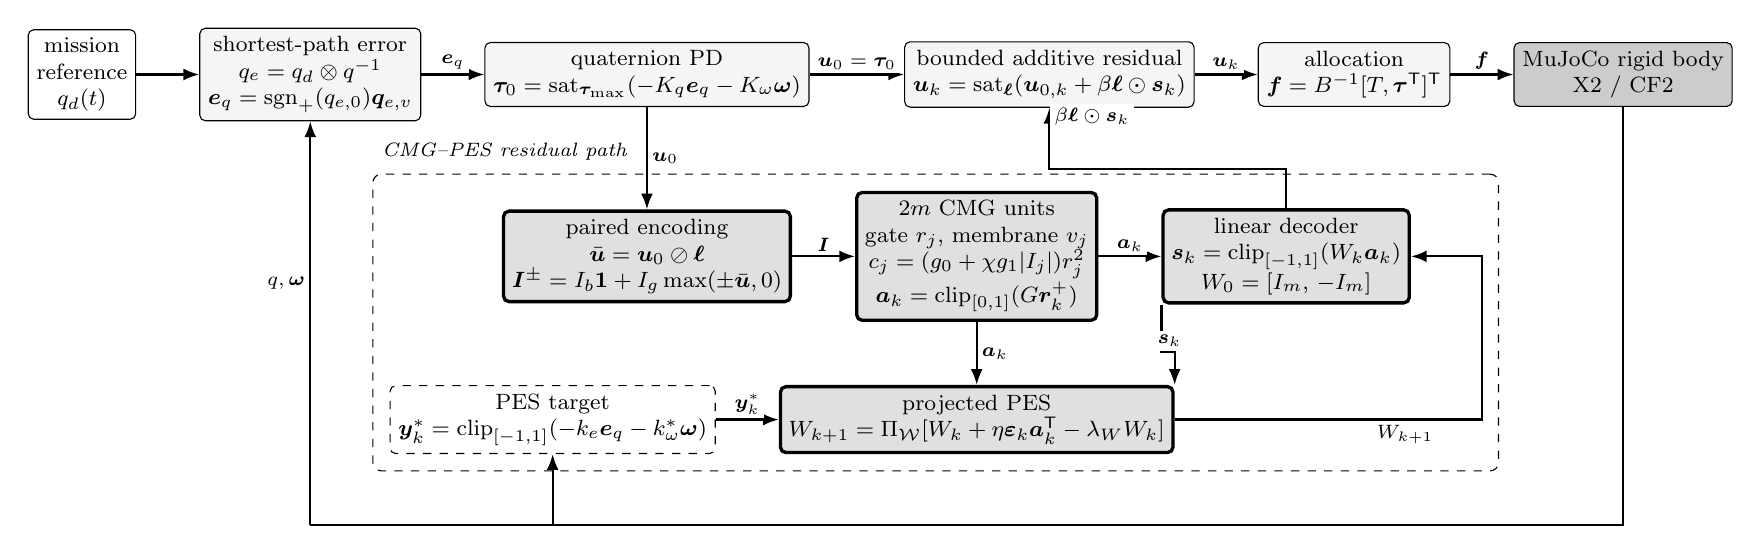
\begin{tikzpicture}[node distance=6mm and 8mm]
  \node[blk]                    (ref)  {mission\\reference\\$q_d(t)$};
  \node[clas,right=of ref]      (err)  {shortest-path error\\
                                        $q_e=q_d\otimes q^{-1}$\\
                                        $\bm e_q=\sgnp(q_{e,0})\bm q_{e,v}$};
  \node[clas,right=of err]      (pd)   {quaternion PD\\
                                        $\bm\tau_0=\sat_{\bm\tau_{\max}}(-K_q\bm e_q-K_\omega\bm\omega)$};
  \node[clas,right=12mm of pd]  (res)  {bounded additive residual\\
                                        $\bm u_k=\sat_{\bm\ell}(\bm u_{0,k}+\beta\bm\ell\odot\bm s_k)$};
  \node[clas,right=of res]      (alc)  {allocation\\$\bm f=B^{-1}[T,\bm\tau\T]\T$};
  \node[plant,right=of alc]     (plt)  {MuJoCo rigid body\\X2 / CF2};

  \node[neuro,below=13mm of pd] (enc)  {paired encoding\\
                                        $\bar{\bm u}=\bm u_0\oslash\bm\ell$\\
                                        $\bm I^{\pm}=I_b\bm 1+I_g\max(\pm\bar{\bm u},0)$};
  \node[neuro,right=of enc]     (cmg)  {$2m$ CMG units\\
                                        gate $r_j$, membrane $v_j$\\
                                        $c_j=(g_0+\chi g_1|I_j|)r_j^2$\\
                                        $\bm a_k=\clip_{[0,1]}(G\bm r_k^{+})$};
  \node[neuro,right=of cmg]     (dec)  {linear decoder\\
                                        $\bm s_k=\clip_{[-1,1]}(W_k\bm a_k)$\\
                                        $W_0=[I_m,\,-I_m]$};
  \node[neuro,below=8mm of cmg](pes)  {projected PES\\
                                        $W_{k+1}=\Pi_{\mathcal W}[W_k+\eta\bm\varepsilon_k\bm a_k\T-\lambda_W W_k]$};
  \node[meas,left=of pes]       (tgt)  {PES target\\
                                        $\bm y^*_k=\clip_{[-1,1]}(-k_e\bm e_q-k^*_\omega\bm\omega)$};

  \draw[sig] (ref) -- (err);
  \draw[sig] (err) -- node[lbl,above]{$\bm e_q$} (pd);
  \draw[sig] (pd)  -- node[lbl,above]{$\bm u_0=\bm\tau_0$} (res);
  \draw[sig] (res) -- node[lbl,above]{$\bm u_k$} (alc);
  \draw[sig] (alc) -- node[lbl,above]{$\bm f$} (plt);

  \draw[sig] (pd.south) -- node[lbl,right]{$\bm u_0$} (enc.north);
  \draw[sig] (enc) -- node[lbl,above]{$\bm I$} (cmg);
  \draw[sig] (cmg) -- node[lbl,above]{$\bm a_k$} (dec);
  \draw[sig] (dec.north) -- ++(0,5mm) -| node[lbl,pos=.93,right]{$\beta\bm\ell\odot\bm s_k$} (res.south);
  \draw[sig] (cmg.south) -- node[lbl,right]{$\bm a_k$} (pes.north);
  \draw[sig] (tgt) -- node[lbl,above]{$\bm y^*_k$} (pes);
  \draw[sig] (dec.south west) -- ++(0,-6mm) -| node[lbl,pos=.3,above]{$\bm s_k$} (pes.north east);
  \coordinate (wx) at ($(dec.east)+(9mm,0)$);
  \draw[sig] (pes.east) -- node[lbl,pos=.75,below]{$W_{k+1}$} (pes.east-|wx) -- (wx) -- (dec.east);

  \coordinate (busy) at ($(pes.south)+(0,-9mm)$);
  \draw[thick] (plt.south) -- (plt|-busy) -- (err|-busy);
  \draw[sig]   (err|-busy) -- node[lbl,pos=.6,left]{$q,\bm\omega$} (err.south);
  \draw[sig]   (tgt|-busy) -- (tgt.south);

  \begin{scope}[on background layer]
    \node[grp,fit=(enc)(cmg)(dec)(pes)(tgt)(wx)] (nb) {};
  \end{scope}
  \node[note,anchor=south west] at ([yshift=0.5mm]nb.north west)
    {CMG--PES residual path};
\end{tikzpicture}
}
\caption{CMG--PES residual architecture. The light blocks are the fixed
classical path: error \eqref{eq:theta}, PD law \eqref{eq:pd}, and
allocation \eqref{eq:mixer} are never adapted. The heavy blocks encode the
clipped baseline as paired currents \eqref{eq:encoding}, evolve $2m$
membrane--gate units \eqref{eq:cmg}, and decode a bounded residual
\eqref{eq:readout} that is \emph{added} to the saturated baseline
\eqref{eq:residual}. Only $W_k$ adapts, through \eqref{eq:pes}; $\beta=0$
recovers the baseline exactly.}
\label{fig:arch}
\end{figure*}

% [v6] fig:scale and fig:models were merged: both showed the same two
% aircraft. The old fig:scale call sites now point here.
\begin{figure*}[t]
\centering
\begin{minipage}[b]{0.24\textwidth}\centering
\includegraphics[width=\linewidth]{\detokenize{all/crazyflie2_cropped (1)}}
\end{minipage}\hfill
\begin{minipage}[b]{0.24\textwidth}\centering
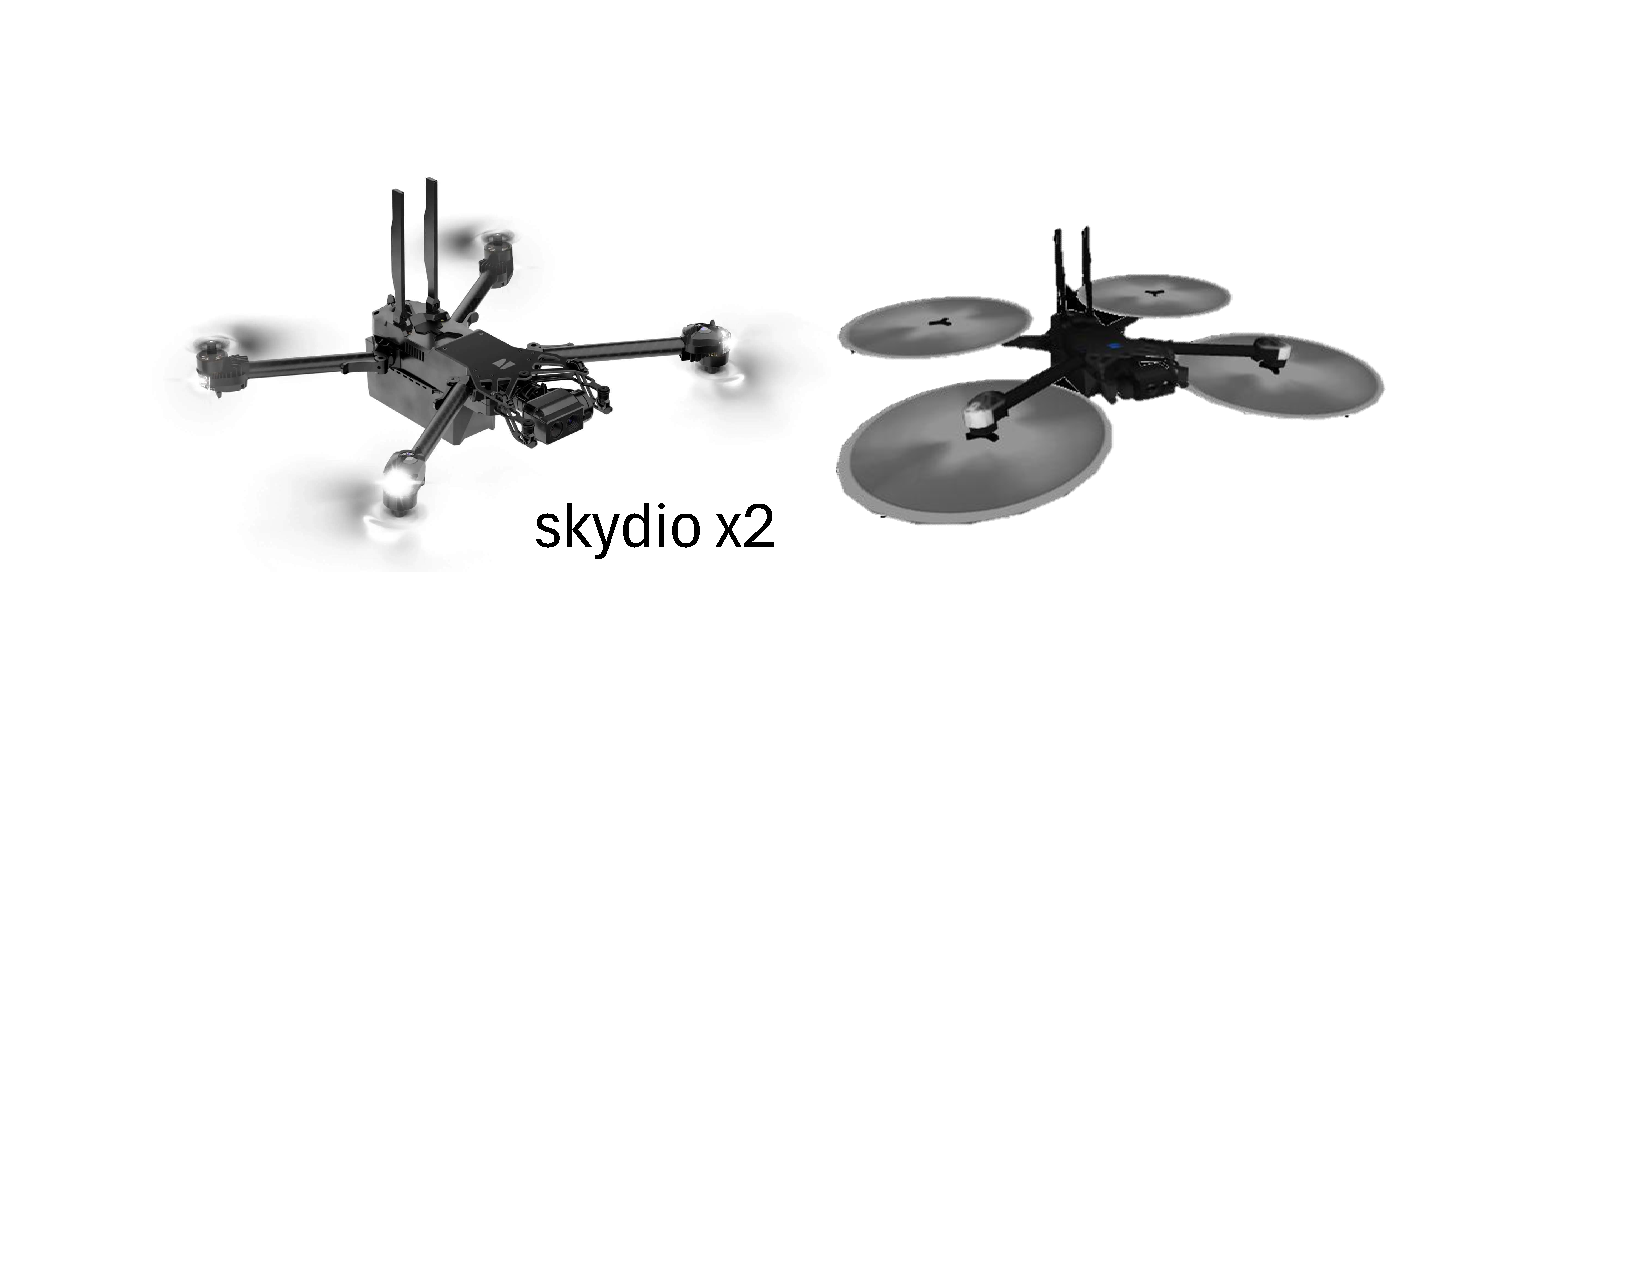
\includegraphics[width=\linewidth]{all/skydiox2_cropped}
\end{minipage}\hfill
\begin{minipage}[b]{0.26\textwidth}\centering
\includegraphics[width=\linewidth]{\detokenize{all/skydio_crazyflie_models_cropped (1)}}
\end{minipage}
\caption{Vehicles and simulation models. Left: CF2 hardware and MuJoCo
model. Centre: X2 hardware and MuJoCo model. Right: both geometries at
relative scale. The axis triads are body-frame axes: they are rigidly
attached to the vehicle and therefore rotate with it relative to the
inertial (world) frame (cf.\ $Q\!:\,\text{body}\to\text{inertial}$ in
Sec.~\ref{sec:problem}).}
\label{fig:models}
\end{figure*}


%%%%%%%%%%%%%%%%%%%%%%%%%%%%%%%%%%%%%%%%%%%%%%%%%%%%%%%%%%%%%%%%%%%%%%%%%%
% [v6] Nomenclature. Every symbol that appears in an equation is listed
% once here; the bracketed tag is the equation that defines it.
\begin{table*}[t]
\caption{Nomenclature. Parenthesised tags give the defining equation;
vectors are bold; $\clip_{[a,b]}$ and $\sat_{\bm\ell}$ act elementwise.}
\label{tab:nomen}\centering\scriptsize
\setlength{\tabcolsep}{4pt}
\renewcommand{\arraystretch}{0.84}
\begin{tabular}{@{}l>{\raggedright\arraybackslash}p{0.185\textwidth}l>{\raggedright\arraybackslash}p{0.185\textwidth}l>{\raggedright\arraybackslash}p{0.185\textwidth}@{}}
\toprule
\multicolumn{6}{@{}l}{\textit{Attitude, plant, and notation}}\\
$q,\;q_d$ & state / reference quaternion & $q_e$ & error quaternion, $q_d\otimes q^{-1}$ & $q_{e,0},\bm q_{e,v}$ & scalar and vector parts\\
$\bm e_q$ & shortest-path error \eqref{eq:theta} & $\theta_q$ & error angle \eqref{eq:theta} & $\bm\omega$ & body angular rate\\
$J$ & inertia tensor & $Q$ & body-to-inertial rotation & $\otimes$ & quaternion product\\
$\bm\omega_d,\bm\omega_e$ & reference and error rate \eqref{eq:errkin} & $R(\cdot)$ & rotation matrix of a quaternion & $z,z_d,\dot z$ & height, reference, rate \eqref{eq:collective}\\
$\odot,\oslash$ & elementwise $\times$, $\div$ & $\sgnp$ & sign, with $\sgnp(0)=1$ & $\sigma$ & logistic function\\
$I_m$ & identity of order $m$ & $\R$ & real numbers & $\Pi$ & Euclidean projection\\
\midrule
\multicolumn{6}{@{}l}{\textit{Fixed baseline and actuator interface}}\\
$\bm\tau_0=\bm u_0$ & baseline torque \eqref{eq:pd} & $K_q,K_\omega$ & PD gains \eqref{eq:pd} & $\bm\tau_{\max}$ & per-axis torque bound\\
$\omega_n,\zeta$ & design frequency, damping & $\bm\ell$ & per-channel command bound & $\sat_{\bm\ell}$ & saturation at $\pm\bm\ell$\\
$B$ & allocation matrix \eqref{eq:allocationmatrix} & $\bm f$ & rotor forces \eqref{eq:mixer} & $T$ & collective thrust \eqref{eq:collective}\\
$\kappa_i$ & rotor reaction coefficient & $m$ & torque channels, $m=3$ & $M$ & vehicle mass\\
$\bm f_{\max}$ & per-rotor force bound & $g$ & gravity, $9.81$\,m/s$^2$ & $\bm 1$ & vector of ones\\
\midrule
\multicolumn{6}{@{}l}{\textit{Coupled membrane--gate unit}}\\
$v_j$ & membrane state \eqref{eq:cmg} & $r_j$ & gate state \eqref{eq:cmg} & $c_j$ & shunt conductance \eqref{eq:cmg}\\
$\bar{\bm u}$ & normalized baseline \eqref{eq:encoding} & $\bm I^{\pm},\bm I$ & paired currents \eqref{eq:encoding} & $I_b,I_g$ & current offset and gain\\
$\tau,\tau_r$ & membrane, gate time constants & $v_{\rm th}$ & gate threshold & $v_{\rm rest},v_{\rm reset}$ & rest level, reversal level\\
$\gamma$ & gate self-coupling & $\alpha_h$ & logistic sharpness & $\chi$ & conductance switch, $\chi\in\{0,1\}$\\
$g_0,g_1$ & conductance gains (distinct from $g$) & $G$ & activity gain, $G=10^5$ & $h$ & integration step\\
$b_{j,k}$ & gate target \eqref{eq:gate_step} & $r^+_{j,k},v^+_{j,k}$ & updated states \eqref{eq:mem_step} & $\lambda_{j,k},d_{j,k}$ & frozen membrane coefficients\\
\midrule
\multicolumn{6}{@{}l}{\textit{Decoder, online learning, and residual authority}}\\
$\bm a_k$ & clipped activity \eqref{eq:readout} & $W_k$ & decoder \eqref{eq:readout} & $W_0$ & initial decoder, $[I_m,-I_m]$\\
$\bm s_k$ & clipped readout \eqref{eq:readout} & $\bm y^*_k$ & PES target \eqref{eq:pes} & $\bm\varepsilon_k$ & PES error \eqref{eq:pes}\\
$k_e,k^*_\omega$ & target gains \eqref{eq:pes} & $\eta$ & per-step learning rate & $\lambda_W$ & per-step decoder decay\\
$\Pi_{\mathcal W},W_{\max}$ & projection and weight bound & $\beta$ & residual authority \eqref{eq:residual} & $\bm u_k,\bm\delta_k$ & applied command, deviation \eqref{eq:residual}\\
\midrule
\multicolumn{6}{@{}l}{\textit{Reported metrics}}\\
$\bar\theta_q$ & mean quaternion-angle error & $S$ & actuator-bound occupancy [\%] & $n$ & runs per reported cell\\
\bottomrule
\end{tabular}
\end{table*}

\section{Simulation Models, Attitude Baseline, and Actuator Interface}
\label{sec:problem}
%%%%%%%%%%%%%%%%%%%%%%%%%%%%%%%%%%%%%%%%%%%%%%%%%%%%%%%%%%%%%%%%%%%%%%%%

\subsection{MuJoCo Platforms and CF2 Actuation Extension}
We use Crazyflie 2.0 (CF2) and Skydio X2 (X2) models derived from MuJoCo
Menagerie \cite{menagerieModels}. Each vehicle has six rigid-body degrees of freedom: three
translations and three rotations, represented by seven free-joint position
coordinates (position and unit quaternion) and six velocity coordinates.
The attitude controller requests three body torques; a separate classical
height loop requests collective thrust. Thus attitude tracking is evaluated
in a freely translating model, not an attitude-only joint model.

The upstream CF2 interface provides collective thrust and three abstract
body-moment channels; its documentation identifies the original actuator
limits as arbitrary and requiring tuning \cite{menagerieCF2}. Our four-rotor actuation extension replaces that
interface with four nonnegative, spatially located thrust inputs while
retaining the source mass, inertia, and visual geometry. Rotor moment arms
and signed reaction-torque coefficients define an explicit allocation
matrix, making the coupling between collective thrust, attitude torque,
and individual actuator limits testable. This is a model-interface
contribution, not a complete aerodynamic identification of CF2.

\begin{table}[!ht]
\centering
\caption{Compiled simulation-model characteristics. CF2 authority is
scaled relative to the upstream model limit, not a manufacturer rating.
Hardware comparisons are given in Table~\ref{tab:manufacturer}.}
\label{tab:models}
\setlength{\tabcolsep}{3pt}
\footnotesize
\begin{tabular}{@{}p{0.40\linewidth}p{0.27\linewidth}p{0.25\linewidth}@{}}
\toprule
Property & CF2 rotor model & X2 model\\
\midrule
Mass $M$ (kg) & $0.027$ & $1.325$\\
Rotor $|p_x|,|p_y|$ (m) & $0.0325,0.0325$ & $0.14,0.18$\\
Reaction magnitude $|\kappa_i|$ (m) & $0.005$ & $0.0201$\\
Unscaled rotor limit (N) & $0.0875$ & $13$\\
Main-test authority scale & $1.5$ & $1$\\
Main-test rotor limit (N) & $0.13125$ & $13$\\
Main-test total limit (N) & $0.525$ & $52$\\
Maximum thrust/weight & $1.321\to1.982$ & $4.001$\\
Rigid-body integrator & RK4 & Euler\\
Experiment timestep (s) & $0.0005$ & $0.0005$\\
Motor activation/RPM states & None & None\\
\bottomrule
\end{tabular}
\end{table}

% [v7] The manufacturer comparison now leads, because it is the fact that
% licenses the model, not an afterthought.
The upstream CF2 model ships without a rotor-level actuation interface, and
its $0.35$ N total thrust limit falls short of the $0.568$ N measured on
stock hardware at $93.75\%$ PWM \cite{bitcrazeThrustMeasurements}. We
therefore complete the model with an explicit four-rotor interface and set
the per-rotor limit so the total is $0.525$ N (Table~\ref{tab:models}),
which remains about $7.5\%$ \emph{below} that measured value. The
correction is toward the manufacturer's own measurement, not beyond it: it
raises modeled maximum thrust/weight from $1.321$ to $1.982$ at
$g=9.81$ m/s$^2$, a figure the physical vehicle exceeds. For physical perspective,
constant-height flight at a single-axis $45^\circ$ tilt requires
$T/(Mg)=1/\cos45^\circ=\sqrt{2}$ even before reserving differential-thrust
margin. The unscaled model cannot meet that idealized requirement; this
does not establish such a limitation for stock CF2 hardware. The scale
changes a simulation thrust bound, not rotor speed, stock propulsion
capability, or tracking performance by $50\%$. Mass, inertia, and reaction
coefficients are unchanged. PD and CMG use the same model and actuator
bounds; any benefit from increased model authority is therefore distinct
from the benefit of neural augmentation.

\begin{table}[!ht]
\centering
\caption{Simulation parameters versus manufacturer information.
``Not reported'' refers to the manufacturer sources reviewed, not proof
that the parameter is unavailable elsewhere.}
\label{tab:manufacturer}
\setlength{\tabcolsep}{3pt}
\footnotesize
\begin{tabular}{@{}>{\raggedright\arraybackslash}p{0.25\linewidth}>{\raggedright\arraybackslash}p{0.30\linewidth}>{\raggedright\arraybackslash}p{0.37\linewidth}@{}}
\toprule
Quantity & Simulation & Manufacturer information\\
\midrule
CF2 mass & $27$ g & $27$ g \cite{bitcrazeCF20Specs}\\
X2 mass & $1325$ g & $1325$ g with battery \cite{skydioX2ESpecs}\\
CF2 total thrust & $0.350\to0.525$ N & $0.568$ N measured at $93.75\%$ PWM\textsuperscript{a} \cite{bitcrazeThrustMeasurements}\\
X2 rotor limit & $13$ N per rotor & Not reported \cite{skydioX2ESpecs}\\
CF2 motor response & No motor dynamics & $\sim180$ ms: $0\to25{,}000$ RPM\textsuperscript{b} \cite{bitcrazeMotorResponse}\\
Inertia tensors & CF2 inherited; X2 geometry-derived & Not reported in product specifications \cite{bitcrazeCF20Specs,skydioX2ESpecs}\\
\bottomrule
\end{tabular}
\par\smallskip
\begin{minipage}{0.97\linewidth}
\scriptsize
\textsuperscript{a}Historical total-thrust measurement with a power-supply
test setup, not a guaranteed continuous battery-powered rating.
\textsuperscript{b}One motor's reported full-command response with a
charged battery; not an identified first-order time constant.
\end{minipage}
\end{table}

The masses agree with published specifications, but this does not
validate all dynamic parameters (Table~\ref{tab:manufacturer}). Bitcraze's
historical measurement of $57.9$ gram-force corresponds to approximately
$0.568$ N; the evaluated $0.525$ N limit is about $7.5\%$ below that
operating point \cite{bitcrazeThrustMeasurements}. This supports a plausible
thrust scale, not hardware validation, and does not establish that a
stronger-than-stock motor is required. CF2 inertia is inherited from
Menagerie, which cites system-identification work \cite{menagerieCF2}; the
rotor-extension moment arms and $|\kappa_i|=0.005$ m remain design
assumptions. X2 inertia, $13$ N rotor limits, and $|\kappa_i|=0.0201$ m are
simulation parameters, not confirmed manufacturer characteristics.

Geometric dimensions also require like-for-like definitions. Bitcraze
lists $92\times92\times29$ mm motor-to-motor/height dimensions
\cite{bitcrazeCF20Specs}; our sites give an opposite-motor separation of
$91.92$ mm. Skydio lists an unfolded flying envelope of approximately
$663\times569\times211$ mm \cite{skydioX2ESpecs}, whereas the model's rotor
centers span $280\times360$ mm. Center spacing and overall flying envelope
are different quantities and do not by themselves establish geometric
agreement or mismatch. Propulsion identification, motor and battery
dynamics, and experimental validation remain necessary for hardware
transfer; no endurance or electrical-power fidelity is claimed.

MuJoCo \cite{todorov2012mujoco} integrates rigid-body motion, gravity, site-applied actuator
wrenches, and enabled passive/contact forces. Both models specify air
density $1.225$ kg/m$^3$ and viscosity $1.8\times10^{-5}$ Pa\,s; their
default inertia-based fluid model \cite{mujocoFluid} is a coarse drag approximation, not
rotor-resolved aerodynamics. The runner overrides the timestep but retains
each model's integrator. Actuators apply algebraic thrust commands without
motor activation dynamics. Although gyro, accelerometer, and orientation
sensors are defined, the evaluated feedback is read directly from
\texttt{qpos}/\texttt{qvel}; optional measurement perturbations are separate
runner settings. These experiments do not establish performance with a
hardware state estimator.

%\input{figure1_interface.tex}

\subsection{Quaternion Convention and Error}
Let $Q\in\mathbb S^3$ be the scalar-first Hamilton quaternion mapping body
coordinates to inertial coordinates, and let $\bm\omega$ be body angular
velocity. With physical inertia $\bm J\succ0$ about the center of mass,
expressed in body axes, the free-flight rotational balance is
\begin{align}
 \dot Q&=\tfrac12 Q\otimes[0,\bm\omega\T]\T,\\
 \bm J\dot{\bm\omega}&=\bm\tau_{\rm act}+\bm\tau_{\rm p}
       +\bm\tau_{\rm d}-\bm\omega\times(\bm J\bm\omega).
 \label{eq:plant}
\end{align}
Here $\bm\tau_{\rm p}$ denotes modeled passive torque and
$\bm\tau_{\rm d}$ any applied disturbance; the nominal ideal rigid-body
model sets both to zero. Contact, if present, contributes an additional
external wrench. The requested torque and actuator torque are distinct
signals in Fig.~\ref{fig:models}.

The controller conjugates MuJoCo's orientation and uses the passive
quaternion $q=Q^{-1}$, so
\begin{equation}
 \dot q=-\tfrac12[0,\bm\omega\T]\T\otimes q.
 \label{eq:passive}
\end{equation}
The desired $q_d$ uses the same convention. Define
\begin{align}
 q_e&=q_d\otimes q^{-1}=[q_{e,0},\bm q_{e,v}\T]\T,\\
 \bm e_q&=\sgnp(q_{e,0})\bm q_{e,v},\qquad \sgnp(0)=1,\\
 \theta_q&=2\operatorname{atan2}(\|\bm q_{e,v}\|_2,|q_{e,0}|)
             \in[0,\pi].
 \label{eq:theta}
\end{align}
The reported error $\theta_q$ is the shortest rotation angle, invariant
under $q_e\mapsto-q_e$. Sign selection introduces a discontinuity at
$q_{e,0}=0$; it does not establish robust hybrid global stability
\cite{mayhew2011hybrid}.
For a desired-frame rate $\bm\omega_d$ satisfying the corresponding
passive kinematics, differentiation gives
\begin{align}
 \dot q_e&=\tfrac12q_e\otimes[0,\bm\omega_e\T]\T,\\
 \bm\omega_e&=\bm\omega-R(q_e)\T\bm\omega_d,\qquad
 \dot q_{e,0}=-\tfrac12\bm q_{e,v}\T\bm\omega_e.
 \label{eq:errkin}
\end{align}
This is a kinematic identity, not a convergence result. Reference Euler
triples parameterize $q_d$ in the passive convention, rather than active
body-to-world Euler commands.

\subsection{Physical Inertia and Implemented PD Gains}
MuJoCo stores principal moments $\bm j_{\rm p}$ in its inertial frame
\cite{mujocoInertial}.
If $R_{BI}$ maps that frame into body axes, the physical inertia is
\begin{equation}
 \bm J=R_{BI}\operatorname{diag}(\bm j_{\rm p})R_{BI}\T.
 \label{eq:inertiaframe}
\end{equation}
The evaluated implementation uses a tuning vector
$\bm j_{\rm tune}=\bm j_{\rm p}$ directly, in the returned array order:
\begin{align*}
 \bm j_{\rm tune}^{\rm CF2}&=(2.3951,2.3951,3.2347)\T10^{-5},\\
 \bm j_{\rm tune}^{\rm X2}&=(0.0607113,0.0364684,0.0254117)\T,
\end{align*}
in kg\,m$^2$. CF2's inertial axes coincide with its body axes. For X2
they do not; its physical body-frame tensor is approximately
\begin{equation}
 \bm J_{\rm X2}=\begin{bmatrix}
 0.0366517&0&-0.0021000\\
 0&0.0254117&0\\
 -0.0021000&0&0.0605280
 \end{bmatrix}\ \mathrm{kg\,m^2}.
\end{equation}
Thus the tuning vector must not be identified with
$\operatorname{diag}(\bm J)$ for both vehicles.

The fixed quaternion PD baseline is
\begin{align}
 \bm k_q&=2\bm j_{\rm tune}\odot\bm\omega_n^2,\qquad
 \bm k_\omega=2\zeta\bm j_{\rm tune}\odot\bm\omega_n,\\
 \bm u_0&=\sat_{\bm\ell}
       (-\bm k_q\odot\bm e_q-\bm k_\omega\odot\bm\omega),
 \label{eq:pd}
\end{align}
where $\odot$ denotes componentwise multiplication,
$\bm\omega_n=(4,4,3.5)\T$ rad/s, $\zeta=0.95$, and
$\sat_{\bm\ell}$ clips component $i$ to $[-\ell_i,\ell_i]$.
For these rotor-interface models, the model-policy torque limits are
$\ell_i=\max(j_{{\rm tune},i}a_i,10^{-6}\ \mathrm{N\,m})$,
with $\bm a=(12,12,10)\T$ rad/s$^2$.
These are controller torque bounds, not guaranteed feasible rotor torques.
The law is quaternion feedback \cite{fresk2013quaternion};
$\bm\omega_n$ parameterizes its gains but is not a verified set of
closed-loop natural frequencies for coupled X2 dynamics.
Desired-rate feedforward and gyroscopic cancellation are omitted.
The identical fixed gains are retained for PD and its CMG augmentation.

For perspective only, take a constant reference, scalar proportional
gain $\bm k_q=k_q\bm1$, the ideal plant
($\bm\tau_{\rm p}=\bm\tau_{\rm d}=0$), no saturation or residual, and a
trajectory confined to one smooth sign branch. Then
$V=\frac12\bm\omega\T\bm J\bm\omega+2k_q(1-|q_{e,0}|)$ gives
$\dot V=-\bm\omega\T\operatorname{diag}(\bm k_\omega)\bm\omega$.
This restricted identity does not prove stability of the anisotropic,
saturated, moving-reference experiments.

\subsection{Requested and Realized Wrench}
For rotor positions $\bm p_i$ in body coordinates, parallel $+z$ thrust
axes, and signed reaction coefficients $\kappa_i$, define
\begin{equation}
 B=\begin{bmatrix}
 1&1&1&1\\p_{1,y}&p_{2,y}&p_{3,y}&p_{4,y}\\
 -p_{1,x}&-p_{2,x}&-p_{3,x}&-p_{4,x}\\
 \kappa_1&\kappa_2&\kappa_3&\kappa_4
 \end{bmatrix}.
 \label{eq:allocationmatrix}
\end{equation}
The signs follow $\bm p_i\times[0,0,f_i]\T$ and the actuator's local
reaction torque $\kappa_i f_i$. Both models have zero body-frame
center-of-mass $x,y$ offsets, so the site's $x,y$ coordinates also give
the relevant center-of-mass moment arms. Figure~\ref{fig:models} fixes the
rotor ordering used by $B$; $\kappa_i$ has units of meters, not angular
velocity. The runner computes
\begin{equation}
 \begin{aligned}
 \bm f_{\rm req}&=B^{-1}[T,\bm u\T]\T,\\
 \bm f_{\rm act}&=\clip_{[\bm0,\bm f_{\max}]}(\bm f_{\rm req}),\\
 [T_{\rm act},\bm\tau_{\rm act}\T]\T&=B\bm f_{\rm act}.
 \end{aligned}
 \label{eq:mixer}
\end{equation}
Here $\bm u=\bm u_0$ for PD; the CMG path in Section~\ref{sec:architecture}
modifies that requested torque before the same allocation and clipping.
Each $f_i$ is a commanded force in newtons, not a rotor-speed command.
Exact wrench realization requires
$B^{-1}[T,\bm u\T]\T\in[\bm0,\bm f_{\max}]$.
A componentwise torque box is not generally contained in this
collective-dependent feasible set. Clipped inverse allocation is used,
not an optimization-based allocator \cite{monteiro2016allocation}.

Collective thrust remains classical, with $z_d=1$ m:
\begin{equation}
 T=\clip_{[0,2.5Mg]}
 \left(\frac{M[g+6(z_d-z)-4\dot z]}{\max(R(Q)_{33},0.35)}\right).
 \label{eq:collective}
\end{equation}
This expression uses the model's $g=9.81$ m/s$^2$. The height loop reads
free-joint height and vertical velocity; the denominator compensates tilt
with a lower guard. Its upper bound does not supersede individual rotor
limits. The CMG path has no direct collective output, but can affect
height through attitude, tilt compensation, and allocation saturation.
The resulting shared plant interface isolates changes in requested
attitude torque while preserving the same physical simulation for both
controllers.

%%%%%%%%%%%%%%%%%%%%%%%%%%%%%%%%%%%%%%%%%%%%%%%%%%%%%%%%%%%%%%%%%
\section{CMG State Dynamics and Online Decoder Adaptation}
\label{sec:architecture}
%%%%%%%%%%%%%%%%%%%%%%%%%%%%%%%%%%%%%%%%%%%%%%%%%%%%%%%%%%%%%%%%%
\subsection{Encoding, States, and Numerical Update}
Symbols are collected in Table~\ref{tab:nomen}.
For $m$ torque channels and $2m$ units, normalize the clipped baseline and
form positive/negative current pairs:
\begin{equation}
 \begin{aligned}
 \bar{\bm u}&=\bm u_0\oslash\bm\ell,\\
 \bm I^{\pm}&=I_b\bm1+I_g\max(\pm\bar{\bm u},\bm0),\\
 \bm I&=[(\bm I^+)\T,(\bm I^-)\T]\T.
 \end{aligned}
 \label{eq:encoding}
\end{equation}
Each unit has a dimensionless membrane state $v_j$ and gate $r_j$:
\begin{align}
 \dot r_j&=[\sigma(\alpha_h(v_j-v_{\rm th}+\gamma r_j))-r_j]/\tau_r,\\
 \dot v_j&=-(v_j-v_{\rm rest})/\tau+I_j/\tau-c_j(v_j-v_{\rm reset}),\\
 c_j&=(g_0+\chi g_1|I_j|)r_j^2,\qquad \chi\in\{0,1\}.
 \label{eq:cmg}
\end{align}
% [v6] CMG unit coupling topology. Source: figures/arch/archB1c.tex
% (editable draw.io version: figures/arch/architectures.drawio, page B1).
\begin{figure}[t]
\centering
\resizebox{0.86\columnwidth}{!}{% B1c -- column-native CMG unit: coupling topology only. The state
% equations stay in the text; the figure shows which variable acts on which.
% Natural width is about one IEEE column, so no \resizebox is needed.
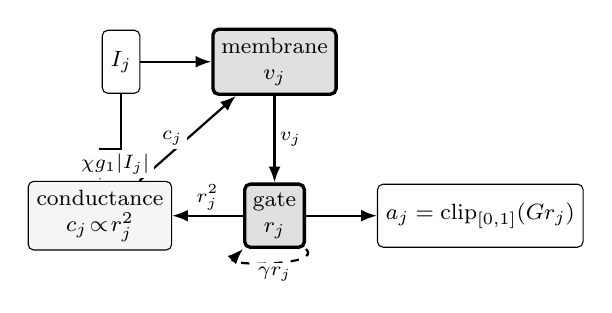
\begin{tikzpicture}[node distance=6mm and 9mm,font=\footnotesize]
  \node[blk]                       (I) {$I_j$};
  \node[neuro,right=of I]          (v) {membrane\\$v_j$};
  \node[neuro,below=11mm of v]     (r) {gate\\$r_j$};
  \node[clas,left=of r]            (c) {conductance\\$c_j\!\propto\! r_j^{2}$};
  \node[blk,right=of r]            (a) {$a_j=\clip_{[0,1]}(G r_j)$};

  \draw[sig] (I) -- (v);
  \draw[sig] (v.south) -- node[lbl,right]{$v_j$} (r.north);
  \draw[sig] (r) -- node[lbl,above]{$r_j^{2}$} (c);
  \draw[sig] (c) -- node[lbl,left]{$c_j$} (v);
  \draw[sig] (r) -- (a);
  \draw[sigd] (r.south east) to[out=-45,in=-135]
        node[lbl,below]{$\gamma r_j$} (r.south west);
  \draw[sig] (I.south) -- ++(0,-7mm) -| node[lbl,pos=.14,below]{$\chi g_1|I_j|$} (c.north);
\end{tikzpicture}
}
\caption{Coupling topology of one CMG unit, cf.~\eqref{eq:cmg}. The
membrane sets the gate target; the gate acts back twice, shifting its own
threshold through $\gamma$ and shunting the membrane through
$c_j\propto r_j^2$ ($\chi=1$ makes that shunt input dependent). The
dynamics are continuous: no spike, no reset, and only $a_j$ leaves the
unit.}
\label{fig:cmgunit}
\end{figure}

The logistic gate target depends on $v_j$, while $r_j$ shifts that target
and modulates membrane conductance (Fig.~\ref{fig:cmgunit}). Thus, both states participate even
though the decoder reads the gate-derived activity. The model has no
threshold-triggered reset or spike event; $v_{\rm reset}$ is a reversal
level in a continuous conductance term. The gains $g_0,g_1$ have the units
needed to make $c_j$ a rate.

The actual integration is sequential, not exponential Euler for both
states. From the old states compute
\begin{align}
 b_{j,k}&=\sigma\!\left(\clip_{[-60,60]}
       [\alpha_h(v_{j,k}-v_{\rm th}+\gamma r_{j,k})]\right),\\
 r_{j,k}^{+}&=\clip_{[0,1]}
       [r_{j,k}+(h/\tau_r)(b_{j,k}-r_{j,k})].
 \label{eq:gate_step}
\end{align}
Then evaluate $c_{j,k}=(g_0+\chi g_1|I_{j,k}|)(r_{j,k}^{+})^2$,
$\lambda_{j,k}=\tau^{-1}+c_{j,k}$, and
$d_{j,k}=(v_{\rm rest}+I_{j,k})/\tau+c_{j,k}v_{\rm reset}$. The
frozen-coefficient membrane step is
\begin{equation}
 v_{j,k}^{+}=e^{-\lambda_{j,k}h}v_{j,k}
       +(1-e^{-\lambda_{j,k}h})d_{j,k}/\lambda_{j,k}.
 \label{eq:mem_step}
\end{equation}
This exactly solves the scalar membrane equation with those frozen
coefficients; it does not establish unconditional stability of the coupled
nonlinear closed loop. Assign $(v_{j,k+1},r_{j,k+1})=(v_{j,k}^{+},r_{j,k}^{+})$.

\subsection{Readout, PES, and Additive Residual}
The within-step activity, initial decoder, and clipped readout are
\begin{equation}
 \begin{aligned}
 \bm a_k&=\clip_{[0,1]}(G\bm r_k^+),\qquad W_0=[I_m,-I_m],\\
 \bm s_k&=\clip_{[-1,1]}(W_k\bm a_k).
 \end{aligned}
 \label{eq:readout}
\end{equation}
Pair subtraction retains directional information from a nonnegative
activity basis; state memory does not imply instantaneous sign agreement
after a command reversal. The teaching target and local update are
\begin{align}
 \bm y_k^*&=\clip_{[-1,1]}(-k_e\bm e_{q,k}-k_\omega^*\bm\omega_k),\\
 \bm\varepsilon_k&=\bm y_k^*-\bm s_k,\\
 W_{k+1}&=\Pi_{\mathcal W}
       [W_k+\eta\bm\varepsilon_k\bm a_k\T-\lambda_W W_k].
 \label{eq:pes}
\end{align}
Here $\mathcal W=[-W_{\max},W_{\max}]^{m\times2m}$, and
$\eta$ and $\lambda_W$ are per-step coefficients, not continuous-time
rates. Holding them fixed while changing $h$ changes the learning dynamics.
PES learns a prescribed residual target; it does not differentiate through
the plant or directly minimize the closed-loop tracking cost. In particular,
with a clipped readout this rule is not the exact gradient of the clipped
instantaneous squared loss. It is a PES-style error-directed update with
projection and leak.

Using $W_k$ before the update, the requested command is
\begin{equation}
 \bm u_k=\sat_{\bm\ell}(\bm u_{0,k}+\beta\bm\ell\odot\bm s_k),\quad
 \bm\delta_k=\bm u_k-\bm u_{0,k},\qquad 0\le\beta\le1.
 \label{eq:residual}
\end{equation}
The canonical UAV case has $m=3$, six CMG units, and eighteen decoder
weights. Intrinsic conductance modulation ($\chi$), synaptic/decoder
adaptation ($W_k$), and output authority ($\beta\bm\ell$) are distinct.

\subsection{Structural Properties and Their Scope}
\begin{proposition}[Bounded internal states]
With the nonnegative conductance parameters in Table~\ref{tab:parameters},
$r_{j,0}\in[0,1]$, and $0<h\le\tau_r$, the gate remains in $[0,1]$.
The membrane iterate remains in the convex hull of its initial value,
$v_{\rm reset}$, and the interval
$[v_{\rm rest}+I_b,v_{\rm rest}+I_b+I_g]$.
\end{proposition}
\begin{proof}
The unclipped gate step is a convex combination of $r_{j,k}$ and
$b_{j,k}\in[0,1]$. Since $I_j\in[I_b,I_b+I_g]$ and $c_j\ge0$,
$d_j/\lambda_j$ is a convex combination of $v_{\rm rest}+I_j$ and
$v_{\rm reset}$. Equation~\eqref{eq:mem_step} is a convex combination of
$v_{j,k}$ and $d_j/\lambda_j$. Induction proves both statements.
\end{proof}

\begin{proposition}[Bounded authority and baseline recovery]
\label{prop:authority}
For $\bm u_{0,k}\in\mathcal U$ and any finite $W_k$,
$\bm u_k\in\mathcal U$ and $|\delta_{k,i}|\le\beta\ell_i$.
If $\beta=0$, the requested baseline command is recovered at every step.
If $W_k=0$ at a particular step, it is recovered at that step, but learning
need not keep $W_{k+1}=0$.
\end{proposition}
\begin{proof}
The outer clip enforces membership in $\mathcal U$. Its componentwise
nonexpansiveness and $\sat_{\ell_i}(u_{0,k,i})=u_{0,k,i}$ give
$|\delta_{k,i}|\le|\beta\ell_i s_{k,i}|\le\beta\ell_i$.
The recovery statements follow by substitution.
\end{proof}
The same allocator and state then give the same actuator output when
$\beta=0$. The proposition does not establish state safety, rotor
headroom, stability, or a bound on tracking improvement. A bounded
adversarial correction can still degrade or destabilize a nonlinear plant.

\begin{proposition}[Decoder bound and restricted contraction]
\label{prop:pes}
If $W_0\in\mathcal W$, then \eqref{eq:pes} keeps $W_k\in\mathcal W$.
If, additionally, the target and a nonzero activity $\bm a$ are fixed,
leak is zero, and readout clipping and projection remain inactive, then
\begin{equation}
 \bm\varepsilon_{k+1}
       =(1-\eta\|\bm a\|_2^2)\bm\varepsilon_k.
 \label{eq:contraction}
\end{equation}
For a nonzero initial error, its norm contracts to zero when
$0<\eta\|\bm a\|_2^2<2$.
\end{proposition}
\begin{proof}
Projection gives the first result. Under the additional conditions,
$(W_{k+1}-W_k)\bm a=\eta\bm\varepsilon_k\|\bm a\|_2^2$;
subtracting this from the fixed target error gives
\eqref{eq:contraction}. The scalar multiplier has modulus less than one
under the stated condition.
\end{proof}
This is the constant-feature PES result \cite{voelker2015pes}, not a
closed-loop convergence theorem. Since $\|\bm a\|^2\le2m$,
$0<\eta<1/m$ is sufficient for that restricted model with nonzero
activity; changing targets, loss of excitation, clipping, and leakage
invalidate a direct application to the experiment. No unique identification
of all decoder weights follows from one fixed regressor.

% [v7] The statement a control audience looks for first. Scoped: it is a
% conditional bound, not a stability theorem, and says so.
\begin{remark}[Scope of a small-gain argument]
\label{rem:smallgain}
Propositions~\ref{prop:authority} and \ref{prop:pes} place the realized
command deviation in a known box, $|\delta_{k,i}|\le\beta\ell_i$, uniformly
in $k$ and independently of what the decoder has learned. If the baseline
loop is input-to-state stable with respect to an additive torque
perturbation, with gain $\gamma(\cdot)$ on that input, then the augmented
loop inherits an ISS estimate with asymptotic bound
$\gamma(\beta\|\bm\ell\|)$, and $\beta$ tunes it continuously to zero. Two
conditions are not discharged here. The perturbation entering the plant is
post-allocation, so the relevant bound is on $B^{-1}$ applied to
$\bm\delta_k$ under rotor saturation, not on $\bm\delta_k$ itself; and the
required ISS gain for the saturated quaternion-PD baseline is not
established in this paper. The architecture therefore supplies the bounded
perturbation such an argument needs, and identifies the two missing
ingredients, without asserting the conclusion.
\end{remark}

\subsection{Nengo Realization}
In Nengo 4.1.0, CMG is a custom non-spiking \texttt{NeuronType} with
probeable membrane and gate states. Constructed currents are injected into
\texttt{ensemble.neurons}; conventional NEF gain/intercept fitting is
bypassed. The result is a direct-current neural basis with a Nengo PES
decoder, not a claim that the full classical controller has been compiled
into an NEF population representation.

With unfiltered activity and $n=2m$, Nengo's update scaling is matched using
$\eta_N=\eta n/h$ and Nengo error $\bm s_k-\bm y_k^*$.
The implementation subtracts $\lambda_WW_k$ using the pre-step weights
and projects after the simulator step. The measured worst relative
mean-error difference across the ten missions is $2.013\times10^{-6}$;
an isolated command test gives approximately $1.05\times10^{-7}$.
These are numerical comparisons over tested trajectories, not bitwise
identity or independent validation of the control hypothesis.

\section{Experimental Protocol and Cross-Mission Results}
\label{sec:results}
\subsection{Models, Parameters, and Measurements}
MuJoCo supplies rigid-body and actuator simulation \cite{todorov2012mujoco}.
The X2 model uses four rotor actuators. The CF2 case is an explicit
four-rotor design with $1.5\times$ nominal upper thrust authority; it is
neither stock-Crazyflie hardware validation nor a validated motor upgrade.
For both rotor models,
$\bm\ell=\max(\operatorname{diag}(J)\odot(12,12,10)\T,10^{-6}\bm1)$
in N\,m, with the maxima taken componentwise.



\begin{table}[t]
\caption{Canonical 3-channel CMG--PES parameters. Neural states/currents
are normalized model variables; learning coefficients are per step.}
\label{tab:parameters}\centering\small
\begin{tabular}{ll}
\toprule
Quantity & Value\\\midrule
$h$, duration & $0.0005$ s, $45$ s\\
$\tau,\tau_r$ & $0.05$ s, $0.005$ s\\
$v_{\rm rest},v_{\rm reset},v_{\rm th}$ & $0,0,1$\\
$v_{j,0},r_{j,0},\chi$ & $0,0,1$\\
$\alpha_h,\gamma,g_0,g_1$ & $50,2,120,30$\\
$I_b,I_g,G$ & $0.75,1.25,10^5$\\
$\beta,\eta,\lambda_W,W_{\max}$ & $0.5,8\times10^{-4},10^{-6},6$\\
$k_e,k_\omega^*$ & $8,0$\\
\bottomrule
\end{tabular}
\end{table}

Each baseline/CMG pair uses the same initial pose/rate, reference, duration,
allocator, model, and timestep. The primary campaign is nominal and
deterministic, with no injected disturbances or sensor noise. One run per
cell is reported; repeated numerical integration of the same deterministic
case is not statistical replication. Learning remains active throughout
evaluation. We report the sample mean $\bar\theta_q$ and relative reduction
$100(\bar\theta_{q,\rm PD}-\bar\theta_{q,\rm CMG})/\bar\theta_{q,\rm PD}$.
Summary metrics use all 90,000 integration samples; most saved plotting
traces retain every tenth sample (5-ms spacing), while the X2 Hard45
trace is full-rate. Thus recomputing a mean from
the decimated plot data need not exactly reproduce the full-rate metric.

The five reference triples are generated as follows (radians):
Roll is $(0.25\sin0.7t,0,0)$; Full3 is
$0.5\sin(t+(0,\pi/2,\pi)\T)$, componentwise. Hard45 is
\begin{equation}
 \begin{bmatrix}
 0.55\sin(0.75t)+0.20\sin(2.10t+0.40)\\
 0.45\sin(0.95t+\pi/3)+0.18\sin(1.75t)\\
 0.65\sin(0.55t+\pi)+0.25\sin(1.35t+0.20)
 \end{bmatrix}.
\end{equation}
Hardstep holds zero for one second, then cycles every two seconds through
the rows of
\begin{equation}
 \begin{bmatrix}
 .75&-.45&.55\\-.65&.55&-.70\\.50&.50&.90\\-.80&-.35&.20
 \end{bmatrix}.
\end{equation}
Yaw360 is $(0,0,2\pi(3\xi^2-2\xi^3))$ with $\xi=t/45$.
The nominal Hover equilibrium is also available, but its essentially zero
error does not support a meaningful percentage comparison.

\subsection{Primary Five-Mission Matrix}
\begin{table}[t]
\caption{Canonical Nengo CMG--PES versus PD: mean quaternion-angle error
[rad], $45$ s, $n=1$ per cell. $S$ is the logged percentage of samples with
at least one rotor command at a bound, PD/CMG. CF2 denotes the $1.5\times$
rotor-authority design, not stock hardware.}
\label{tab:mujoco}\centering\scriptsize
\setlength{\tabcolsep}{3pt}
\begin{tabular}{llrrrr}
\toprule
Model&Mission&PD&CMG--PES&Reduction&$S$ [\%]\\\midrule
X2&Roll&.050565&.041785&17.36\%&0/0\\
&Full3&.303275&.131748&56.56\%&0/0\\
&Hard45&.294082&.138007&53.07\%&0/0\\
&Hardstep&.454528&.359355&20.94\%&.016/.239\\
&Yaw360&.075863&.029902&60.58\%&0/0\\\midrule
CF2&Roll&.051337&.042439&17.33\%&0/0\\
&Full3&.288383&.126476&56.14\%&0/0\\
&Hard45&.285449&.132319&53.65\%&0/0\\
&Hardstep&.426182&.347886&18.37\%&.137/.264\\
&Yaw360&.075812&.029870&60.60\%&0/0\\\bottomrule
\end{tabular}
\end{table}
All ten primary cases improve mean error (Table~\ref{tab:mujoco}). Gains
are largest on Yaw360 and Full3 and smallest on Roll; the abrupt Hardstep
case is intermediate. The reported bound-occupancy statistic detects
post-clipping commands within the runner's tolerance of a limit. It is not
a measurement of requested-wrench infeasibility magnitude. Hardstep has
small but nonzero occupancy on both models, so a blanket zero-saturation
claim would be incorrect. These cases establish repeatable nominal performance; robustness to model
mismatch and comparison against other baseline families are separate
questions, addressed in Sec.~\ref{sec:conclusion}. Figures~\ref{fig:tracking} and \ref{fig:hard45_neurons} show
the X2 Hard45 case, the largest smooth-mission gain, together with the
neural activity that produced it. Hardstep, the smallest reduction and the
only case with nonzero bound occupancy, is reported in
Tables~\ref{tab:mujoco} and \ref{tab:noise}.

\begin{figure}[t]
\centering
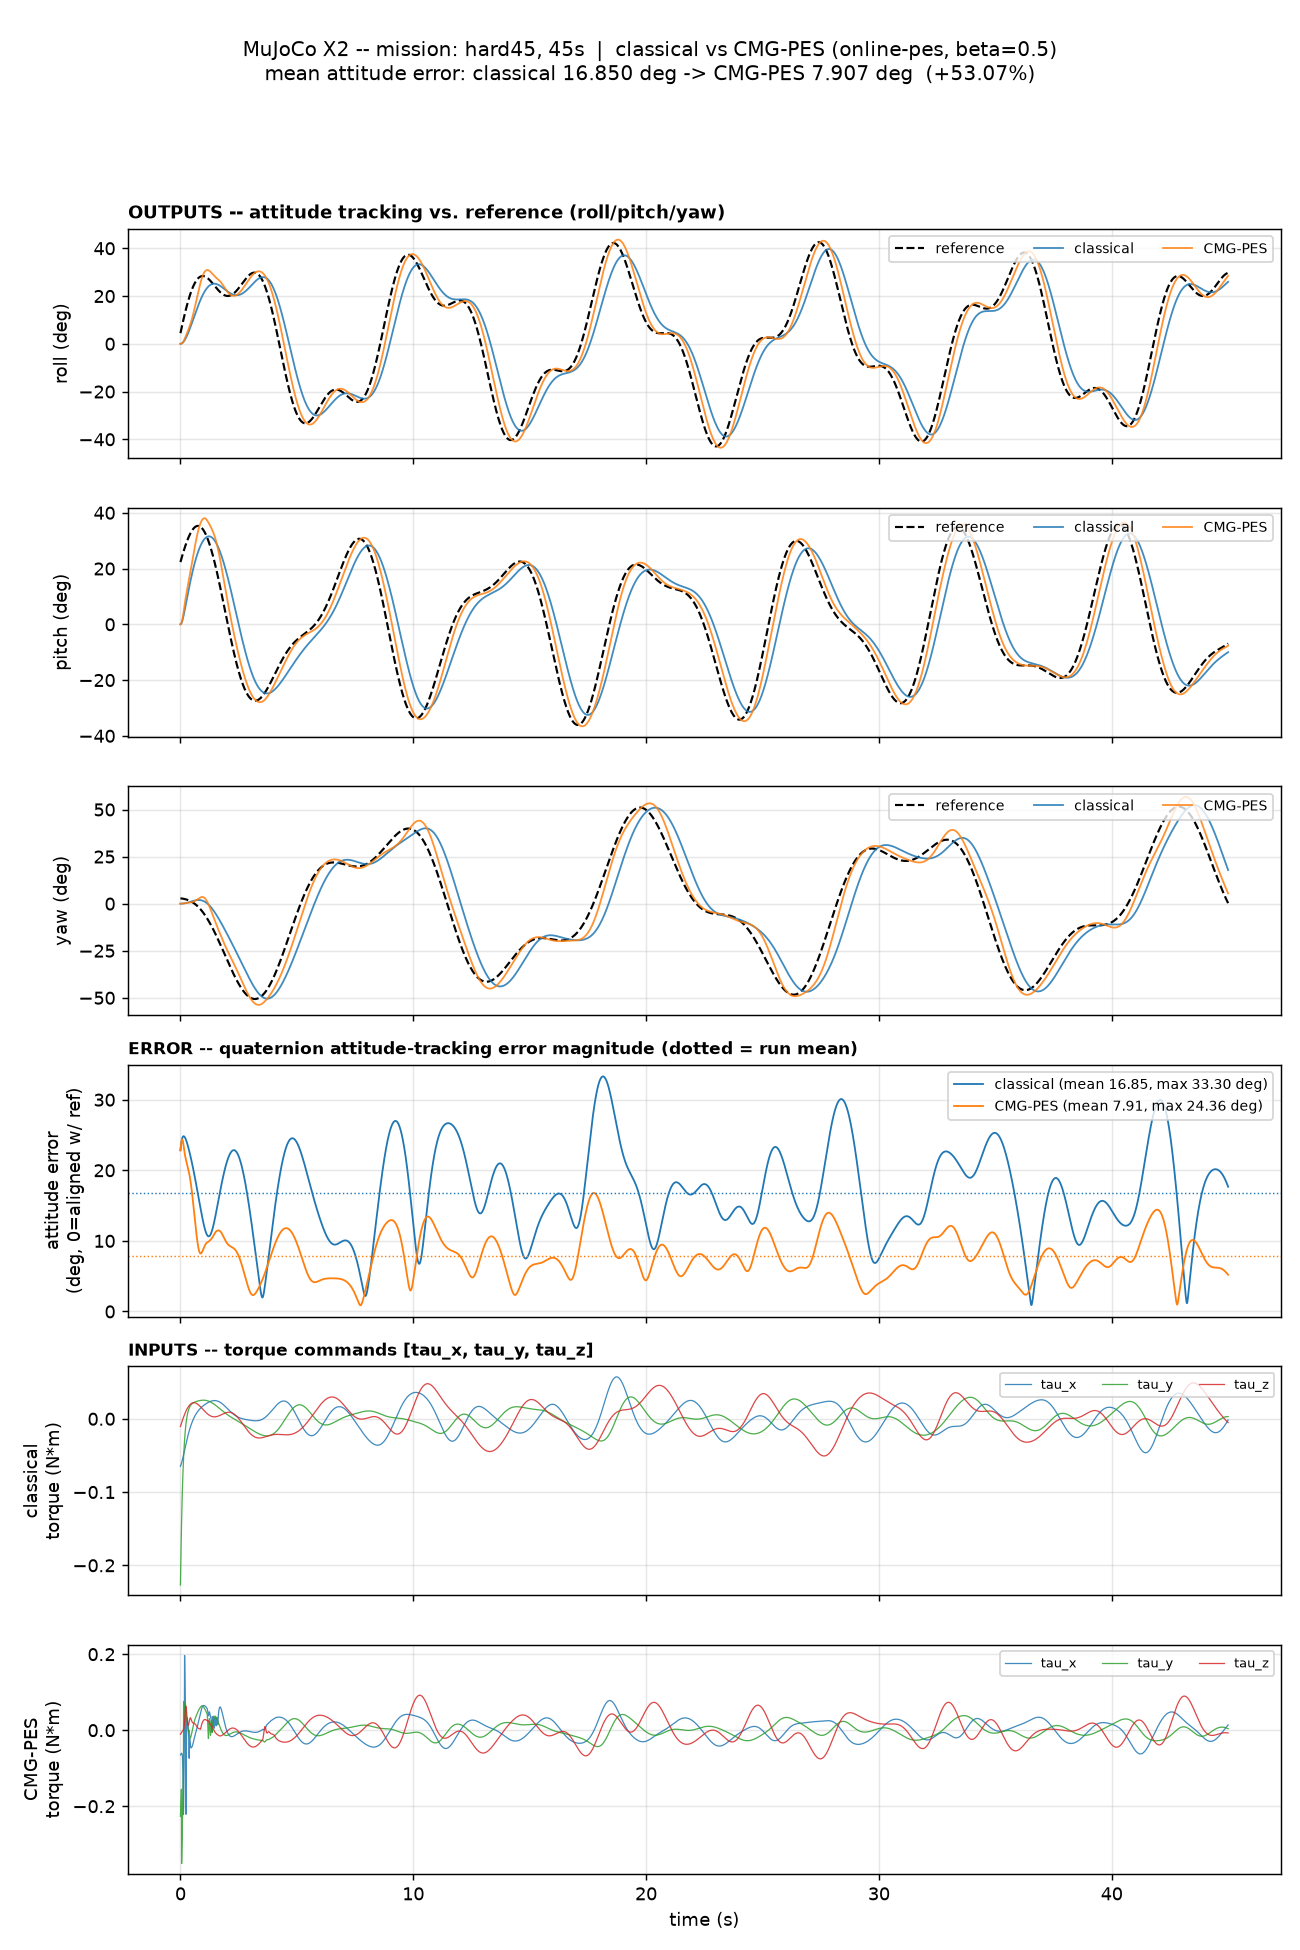
\includegraphics[width=0.62\linewidth]{X2/Hard45/x2_hard45_classical_vs_cmg}
\caption{X2 Hard45: classical baseline vs. CMG--PES residual control.}
\label{fig:tracking}
\end{figure}

\begin{figure}[t]
\centering
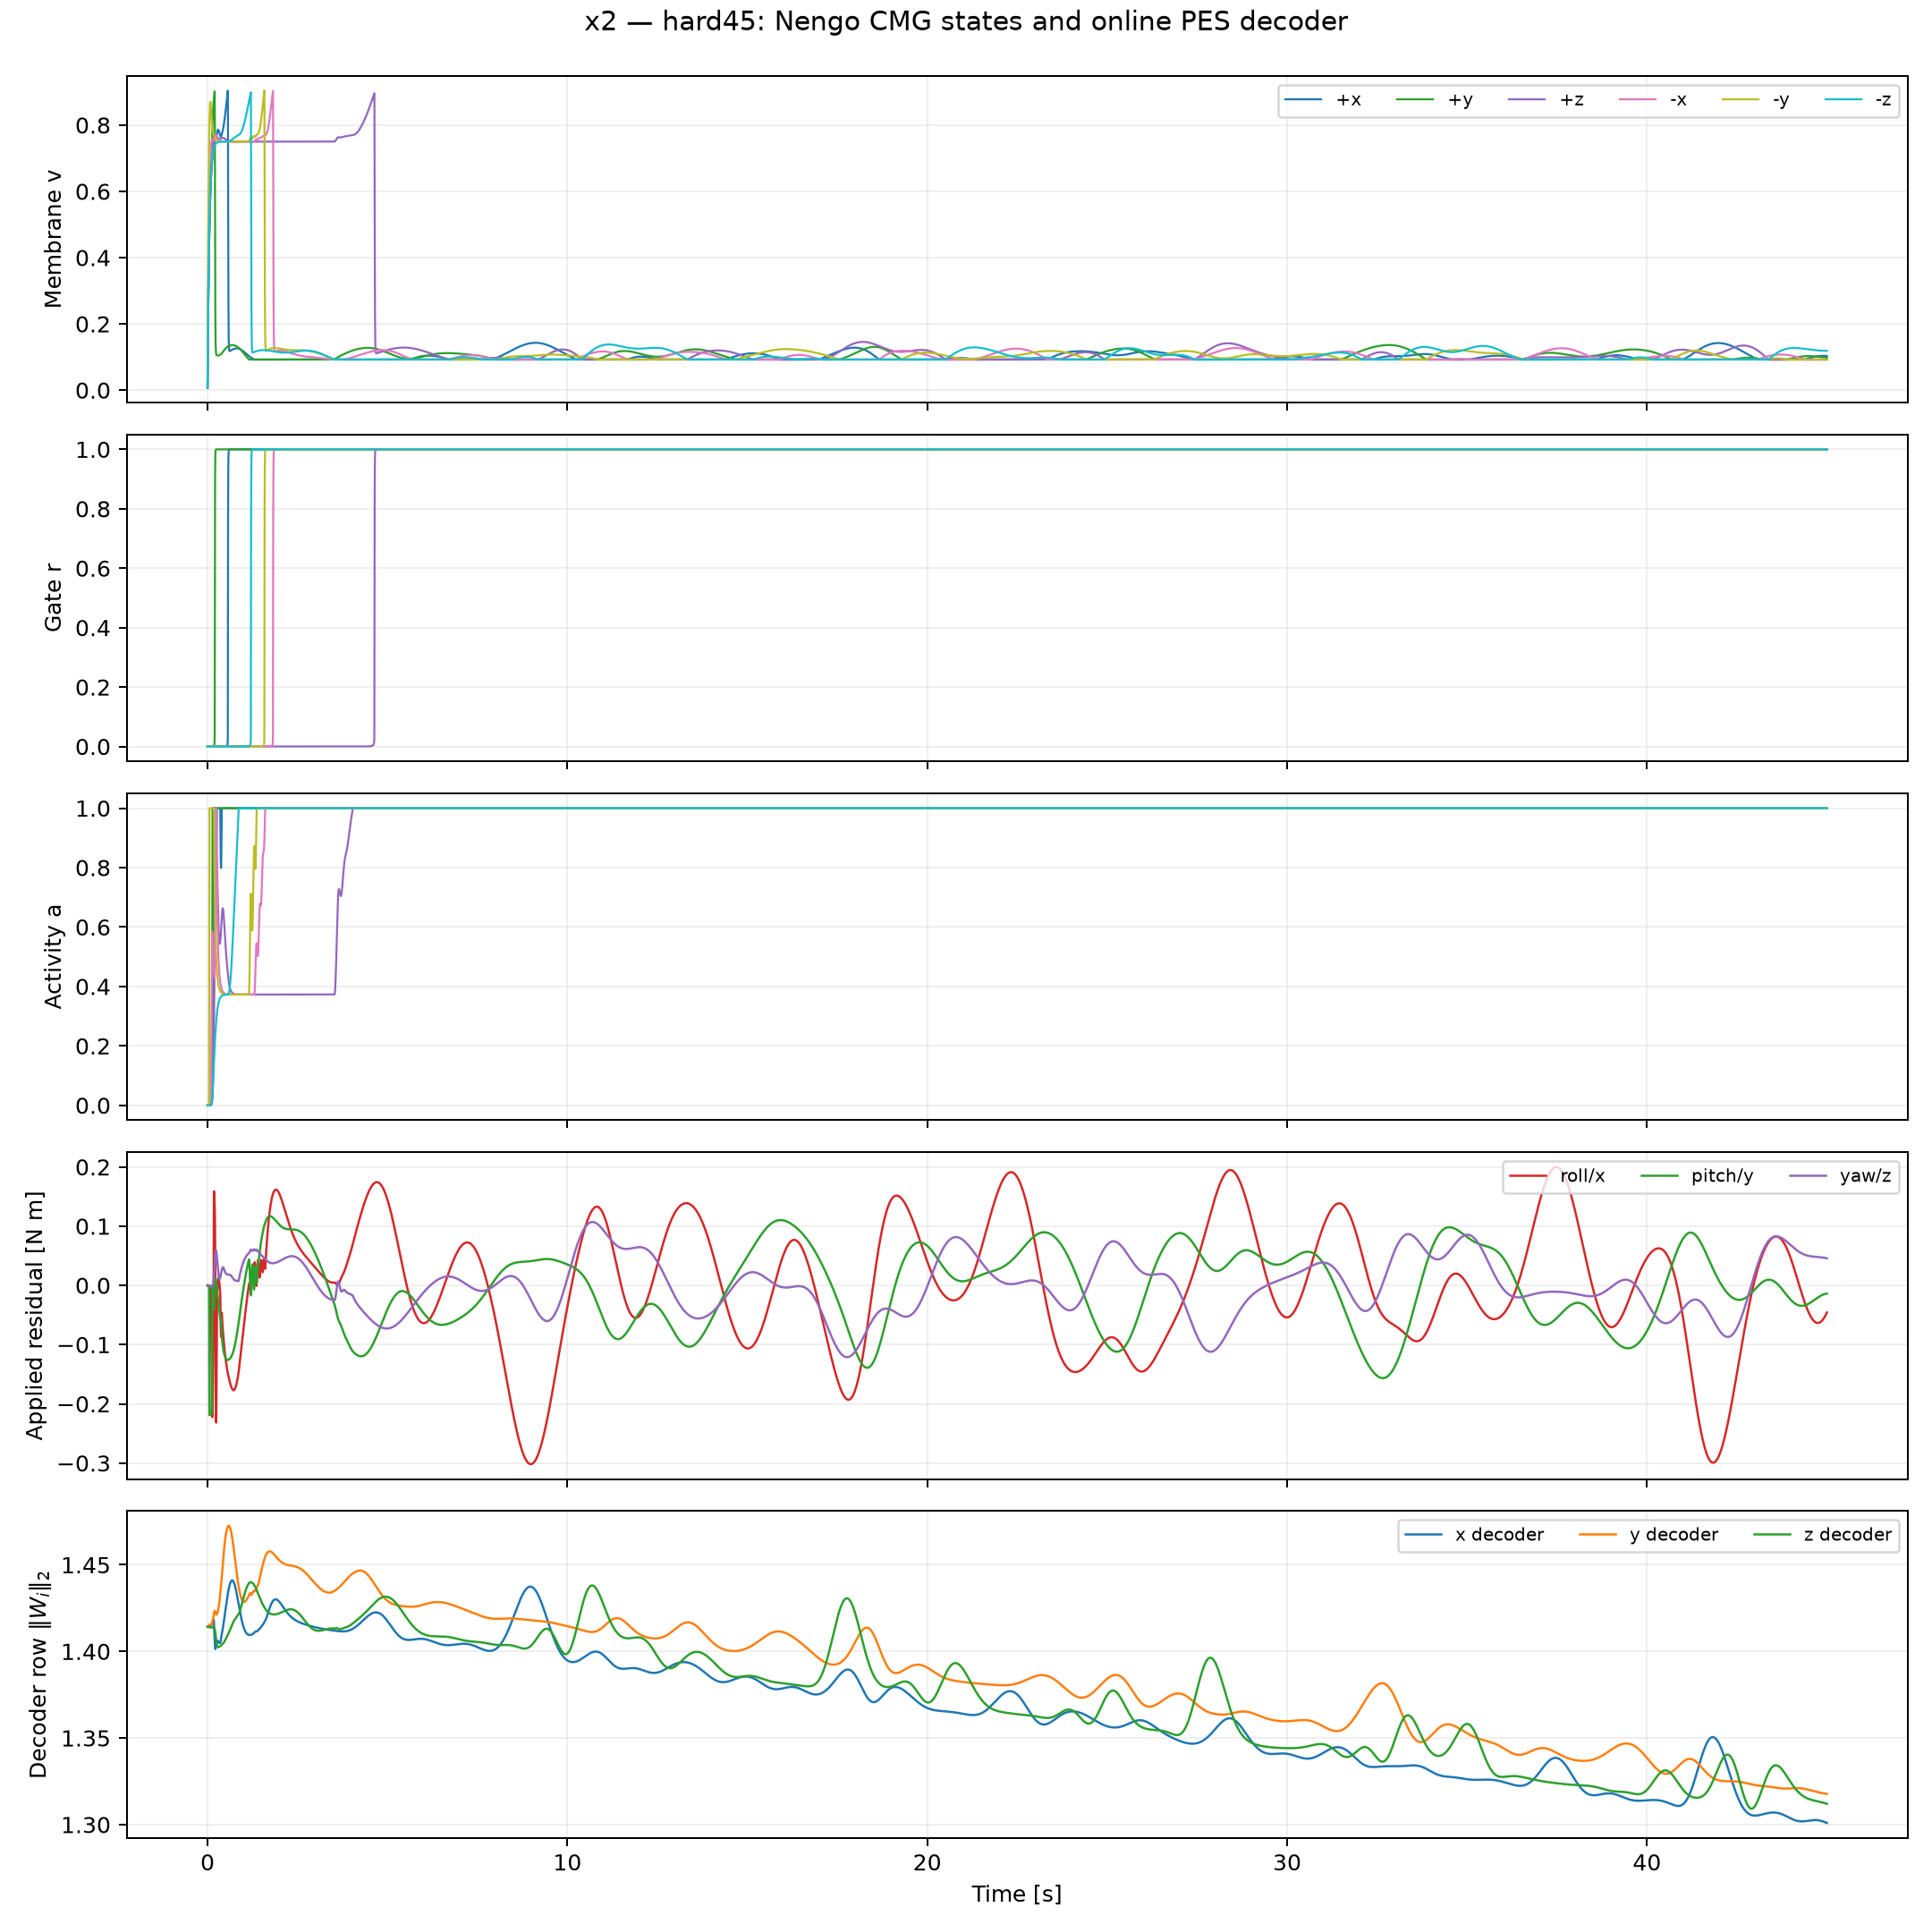
\includegraphics[width=0.62\linewidth]{X2/Hard45/x2_hard45_neurons}
\caption{X2 Hard45: neural activity for the CMG residual controller.}
\label{fig:hard45_neurons}
\end{figure}


% [v8] Noise sensitivity. Generated by compile_final_sweep.py; regenerate
% from results/final_sweep_2026-09-05/compiled/table_noise.tex.
\begin{table}[t]
\caption{Mean-error reduction versus PD under measurement noise. Entries are X2/CF2. Clean
reproduces Table~\ref{tab:mujoco}; moderate is $0.010$\,rad and
$0.025$\,rad\,s$^{-1}$, realistic is $0.020$\,rad and $0.050$\,rad\,s$^{-1}$
on the attitude and rate estimates. Noisy entries average two seeds; the
seed standard deviation is given for the realistic level.}
\label{tab:noise}\centering\scriptsize
\setlength{\tabcolsep}{4pt}
\begin{tabular}{lrrr@{\,}l}
\toprule
Mission&Clean&Moderate&\multicolumn{2}{c}{Realistic}\\\midrule
Roll&17.4/17.3\%&32.3/32.4\%&32.2/32.5\%&$\pm$0.01\\
Full3&56.6/56.1\%&56.4/55.9\%&55.7/55.2\%&$\pm$0.00\\
Hard45&53.1/53.6\%&52.9/53.4\%&52.3/52.7\%&$\pm$0.01\\
Hardstep&20.9/18.4\%&20.8/18.3\%&20.6/18.1\%&$\pm$0.02\\
Yaw360&60.6/60.6\%&56.8/56.8\%&47.8/47.8\%&$\pm$0.03\\
\bottomrule
\end{tabular}
\end{table}

\subsection{Sensitivity to Measurement Noise}
\label{sec:noise}
Table~\ref{tab:mujoco} uses noise-free feedback and one run per cell.
Every cell was therefore rerun with zero-mean Gaussian noise on the attitude
and rate estimates, at two levels and two seeds (Table~\ref{tab:noise}).

Across the twenty noisy cells the seed standard deviation of the reduction
is $0.002$--$0.031\%$, three orders of magnitude below the effect: under
this disturbance model the missions are effectively deterministic, and noise
\emph{magnitude}, not seed, is the axis that matters. The magnitude response
is not uniform. Full3, Hard45, and Hardstep move by under one point. Yaw360
loses $12.8$ points on both models: its absolute error is the smallest in the
matrix, so a fixed noise floor takes a larger share of the ratio. Roll moves
the other way, $17.4\%$ to $32.2\%$, consistent with the residual having more
to correct once the baseline is disturbed. The realistic-noise range is
$18.1$--$55.8\%$, narrower at both ends than $17.3$--$60.6\%$.

\subsection{What Is Learning?}
Fixed-decoder residuals already improve some missions: in the audited direct
X2 runs their mean reductions range from about 0.12\% to 10.27\%; the
corresponding CF2-design range is 0.06\% to 6.80\%. Thus it is inaccurate
to say that fixing the decoder removes \emph{all} improvement. PES produces
the much larger 17.3--60.6\% primary reductions. Separately, toggling
$\chi$ with the decoder mode held fixed is numerically indistinguishable
under the tested settings. Decoder adaptation is therefore the principal lever in the tested regime.

Because $a_j=\clip(10^5r_j,0,1)$, decoder activity saturates already at
$r_j=10^{-5}$. Tiny but nonzero gates can therefore yield order-one
activity while $c_j\propto r_j^2$ remains small. This is a plausible
mechanistic explanation for the observed conductance insensitivity, not
a claim that every gate remains $O(10^{-6})$ at every instant. A calibrated
gate-gain sweep and gate/membrane readout ablation are needed to determine
whether CMG offers benefits beyond a simpler dynamical basis.

\begin{figure}[t]
\centering
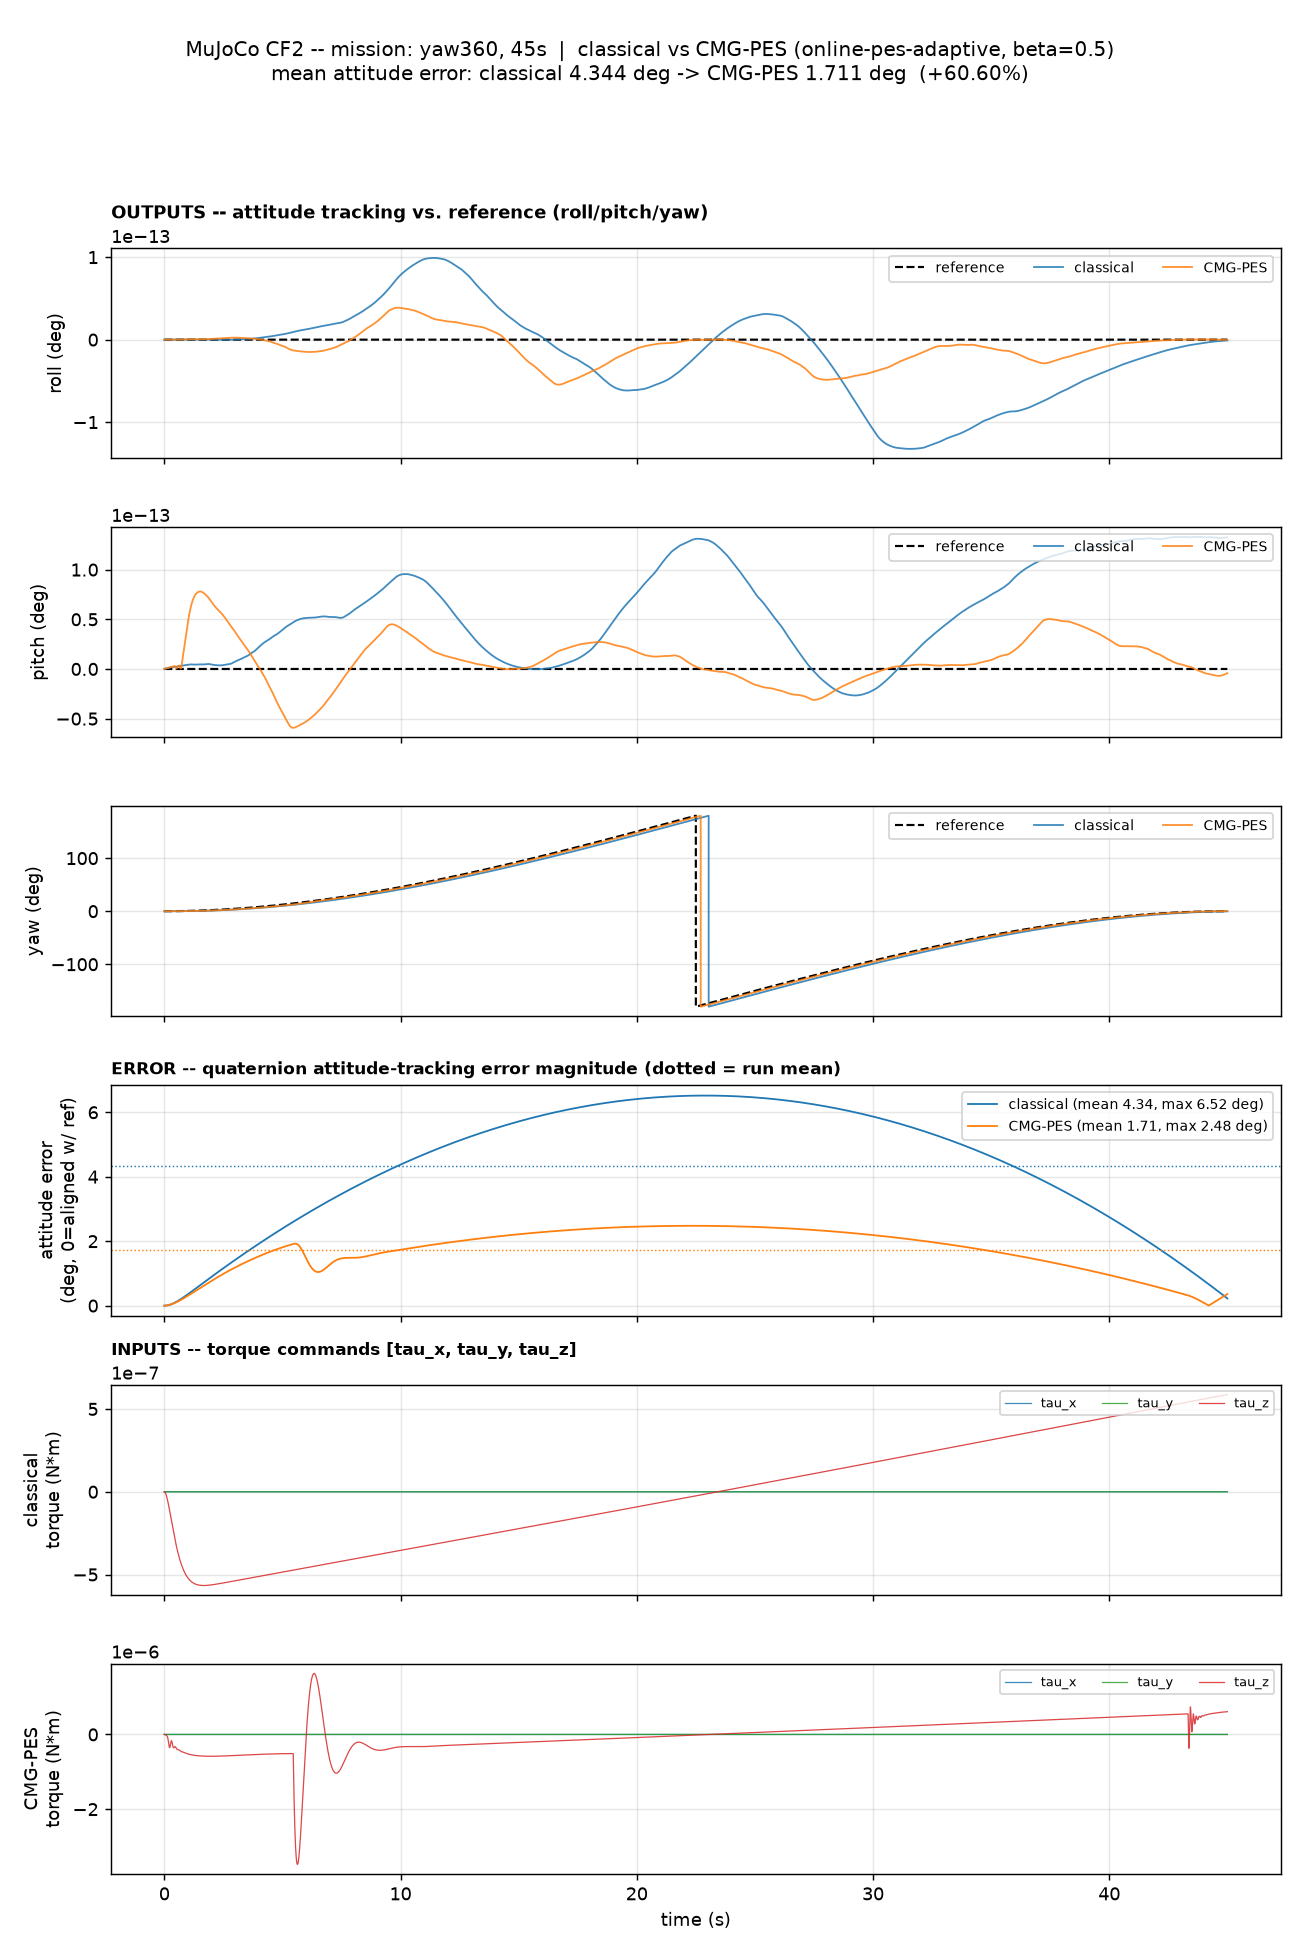
\includegraphics[width=0.62\linewidth]{CF2/Yaw360/cf2_yaw360_classical_vs_cmg}
\caption{CF2 Yaw360: classical baseline vs. CMG--PES residual control.}
\label{fig:states}
\end{figure}

\begin{figure}[t]
\centering
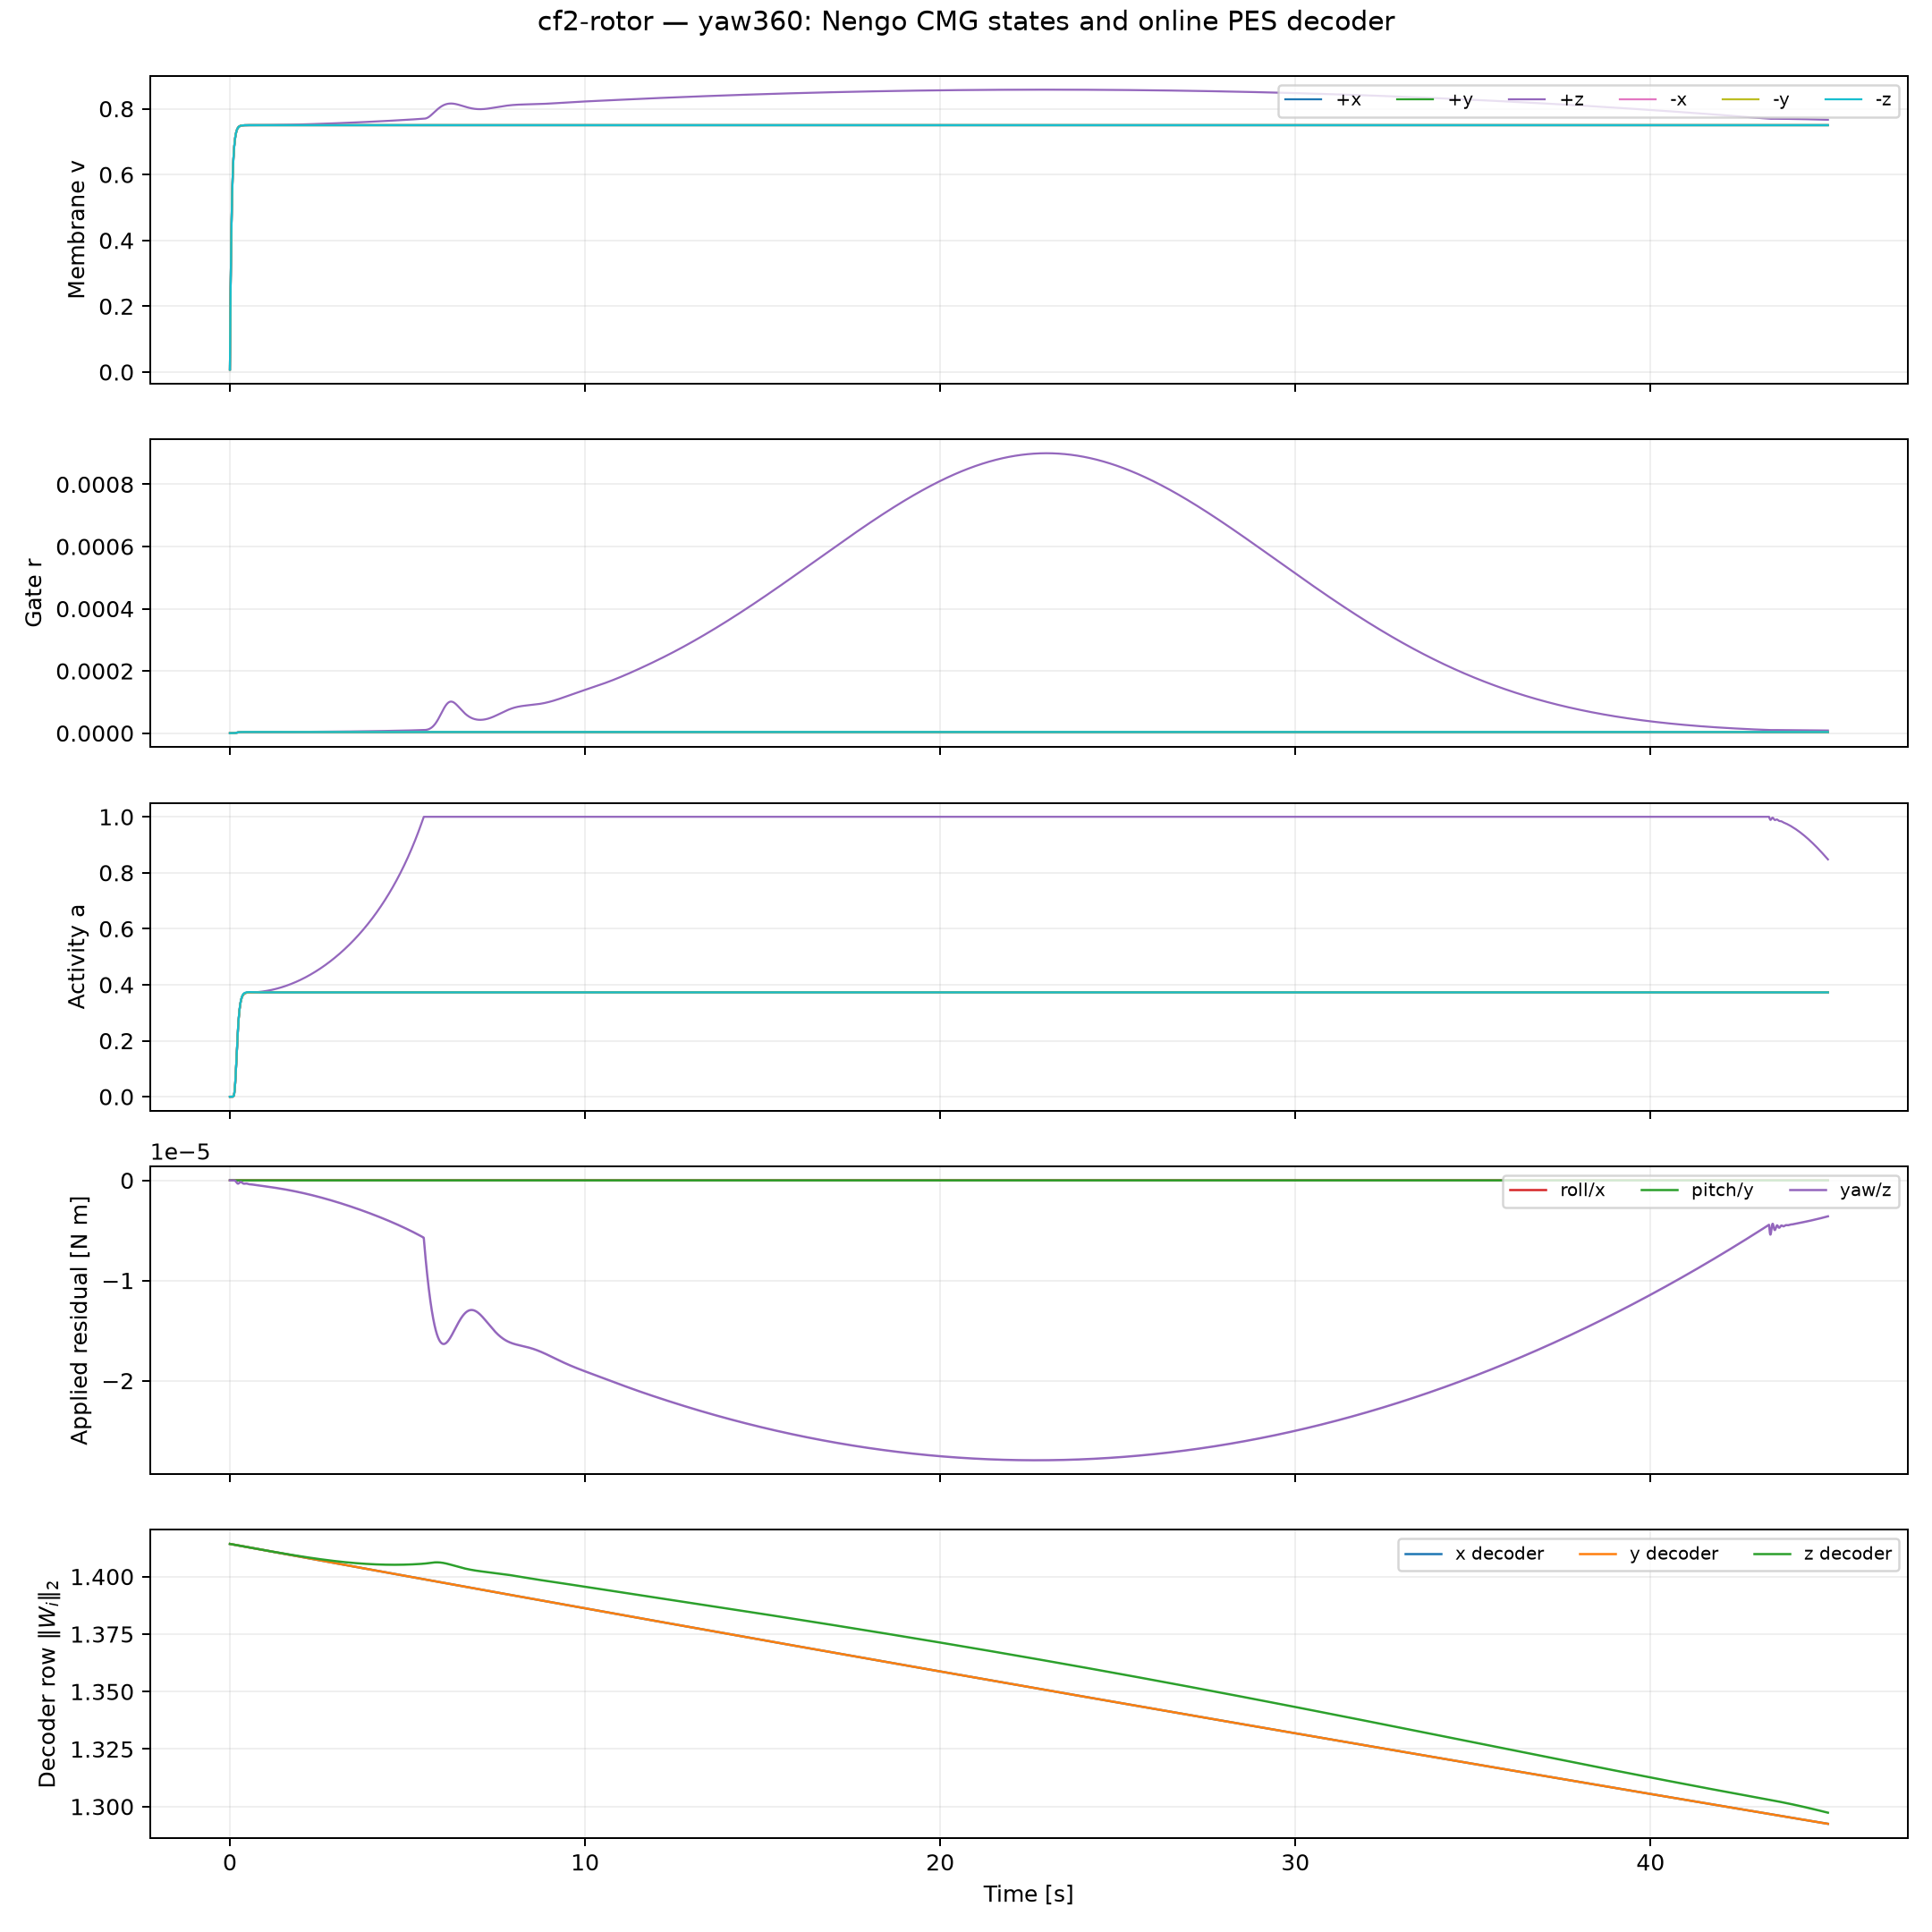
\includegraphics[width=0.62\linewidth]{CF2/Yaw360/cf2-rotor_yaw360_neurons}
\caption{CF2 Yaw360: neural activity for the CMG residual controller.}
\label{fig:cf2_yaw360_neurons}
\end{figure}

Figure~\ref{fig:states} shows the CF2 Yaw360 case, the largest reduction
in Table~\ref{tab:mujoco}, and Fig.~\ref{fig:cf2_yaw360_neurons}
distinguishes the membrane, raw gate, and clipped activity using that same
recorded trajectory rather than equating them.


% [v8] Disturbance rejection. Sources:
% results/hover_intermittent_2026-09-05/ and final_sweep_2026-09-05/B_long_hover.
\begin{figure}[t]
\centering
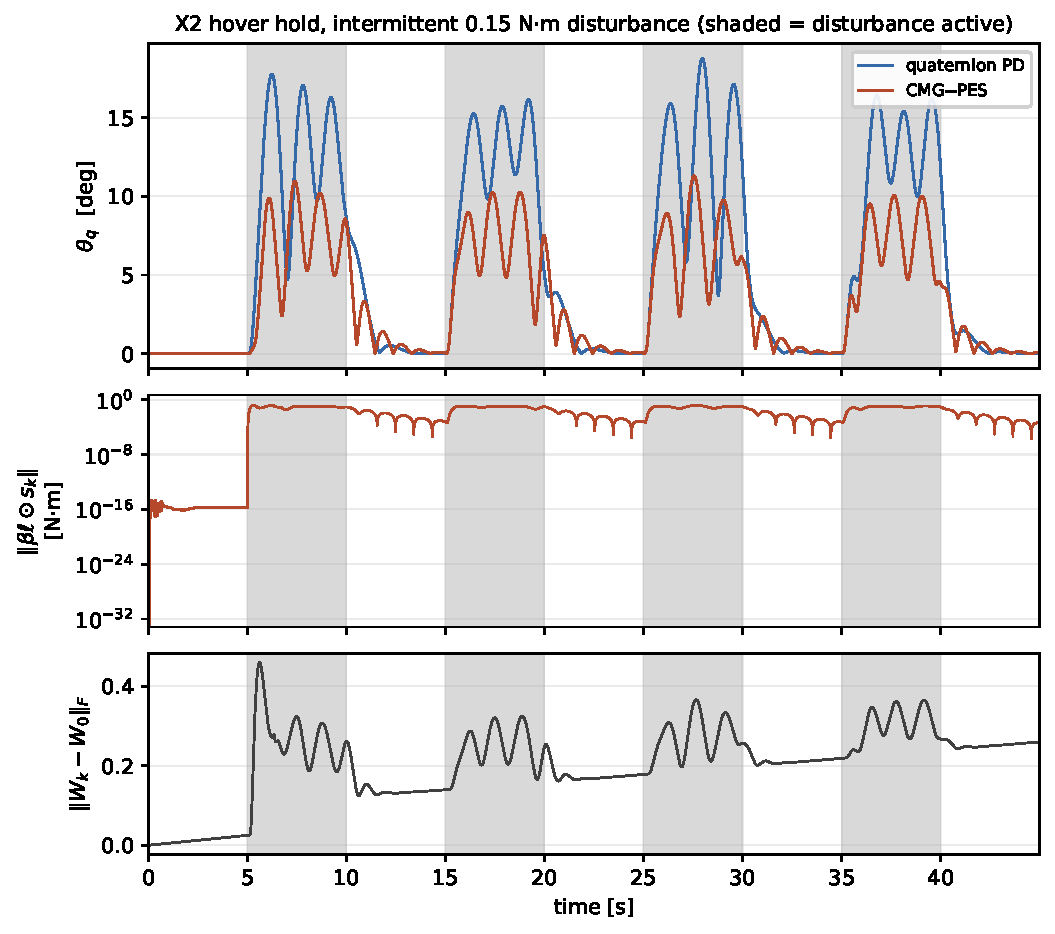
\includegraphics[width=0.78\linewidth]{hover_intermittent}
\caption{X2 hover hold under four $0.15$\,N\,m disturbance bursts (shaded)
separated by quiet intervals. Top: attitude error. Centre: residual
magnitude, logarithmic. Bottom: decoder displacement from $W_0$. The
residual is at machine precision before the first burst, so the augmented
loop costs nothing while the baseline is already exact.}
\label{fig:hover_int}
\end{figure}

\subsection{Disturbance Rejection and Retention}
\label{sec:disturbance}
A complementary test holds the equilibrium attitude and applies a
multi-sine body torque in bursts, so the controller is seen entering a
disturbance, adapting inside it, and then holding a decoder adapted to a
disturbance that has stopped (Fig.~\ref{fig:hover_int}).

Before the first burst the residual norm is $O(10^{-16})$: the augmented
loop is inert when the baseline is already exact. During bursts the mean
error falls from $11.50^\circ$ to $6.65^\circ$ ($42.2\%$), and during the
quiet intervals from $1.21^\circ$ to $0.99^\circ$ ($18.0\%$). The same study
on CF2, with the disturbance scaled by the inertia ratio, gives $50.2\%$.

Over $180$\,s and sixteen bursts the burst-phase reduction stays flat
($43.3\%$ to $40.6\%$) while the quiet-phase reduction improves from
$25.6\%$ to $63.4\%$ and $\|W_k-W_0\|_F$ grows from $0.14$ to $0.75$. The
decoder accumulates a correction reused across episodes rather than
relearning each one. Two caveats: in the second episode the augmented loop
is $4\%$ \emph{worse} in the quiet phase, the only such interval observed;
and the displacement is still growing at $180$\,s, with
$\max_i|W_{k,i}|=1.09$ inside $\mathcal W$ but not saturated, so retention is
not shown to converge on longer missions.

\subsection{Neuron-Family Comparison}
The Nengo benchmark contains two models, five missions, and eleven
controllers: PD and fixed/PES variants of CMG, LIF, ALIF, Izhikevich
\cite{izhikevich2003}, and LIFRate. All use the same residual/allocator
path, with model-specific native activity and filtering. Some
Izhikevich--PES cells outperform CMG--PES on mean tracking error. The audit
reports an approximate average normalized residual RMS of 0.37 for
Izhikevich--PES versus 0.12 for CMG--PES, alongside more decoder movement.
Equal output caps do not imply equal realized correction effort.
Very sparse LIF/ALIF activity in some tested cells is an operating-point
limitation, not evidence that those neuron families cannot learn.
The supported conclusion is therefore a tracking--effort tradeoff: CMG--PES
attains comparable tracking at markedly lower realized residual effort.

\section{Discussion and Conclusion}
\label{sec:conclusion}
% [v7] Rewritten: states the positive result once and plainly, keeps the
% limits in one place instead of after every sentence, and separates the
% analog outlook from the claims.
A fixed quaternion-PD law augmented by six paired continuous membrane--gate
units and eighteen online-adapted decoder weights reduces mean attitude
error by $17.3$--$60.6\%$ across ten matched 45-s cases on two modeled
platforms, with actuator bounds respected throughout and the baseline
recovered exactly at zero authority. The direct and Nengo realizations agree
to $2.013\times10^{-6}$, so the result is a property of the architecture
rather than of one implementation.

The ablation is the more informative half. Holding the decoder mode fixed
and toggling conductance modulation is numerically indistinguishable under
the tested settings, while freezing the decoder removes most of the gain.
In this regime the improvement is carried by online decoder adaptation over
a bounded nonlinear basis, not by the specific neuron dynamics. Because
$a_j=\clip(10^5r_j,0,1)$, activity saturates once $r_j$ exceeds $10^{-5}$,
which plausibly explains that insensitivity and identifies the gate gain as
the parameter a follow-up should sweep first. Reporting this constrains the
architecture's claim rather than supporting it, and it is the reason the
contribution is stated as a controlled separation of mechanisms.

Three limits bound the above. The study is in simulation: the noise
sweep of Sec.~\ref{sec:noise} bounds sensitivity to measurement error and
shows the missions are effectively deterministic under it, but it does not
address model mismatch, and retention in Sec.~\ref{sec:disturbance} has not
converged by $180$\,s. The comparison is against a well-tuned PD without
integral action, not against every reasonable baseline. And bounded
commands, states, and weights are implementation properties, not stability
proofs; Remark~\ref{rem:smallgain} states exactly which two ingredients an
ISS argument still needs.

The continuous regime suggests a hardware direction that a spiking
formulation forecloses. Membrane leak, sigmoidal gating, and a shunting
conductance are the primitives analog neuromorphic circuits implement as
device physics \cite{mahowald1991vlsi}, with no comparator, reset, or
event-routing logic, and the gate transient carries the timing information a
spike would otherwise discretize. Whether that translates into an energy
advantage is untested and does not follow from these results: a graded
analog system draws static rather than event-sparse power, and at six
neurons and eighteen weights the controller is negligible on any substrate.
The claim such a study would have to make is a per-decision energy
comparison at matched tracking accuracy, including conversion and sensing;
online decoder adaptation is attractive there mainly because it can absorb
device mismatch, which is the standard argument for learning on analog
hardware. We flag this as motivation for the continuous formulation, not as
a result.

Preliminary real-time tests on a Quanser 3DOF Hover confirm the controller
meets a 200-Hz hardware deadline with ten 0.5-ms neural substeps per sample;
three matched Roll pairs improved mean error by $2.65\%\pm1.08\%$. That rig
is a different plant from either simulated airframe, so those runs are
reported as feasibility rather than validation and are analyzed separately.
Follow-up work includes an integral-action baseline, a matched-effort
comparison against non-neural bounded bases, a gate-gain sweep, longer
disturbance horizons to test whether retention saturates against
$\mathcal W$, and frozen-weight held-out tests.

% Finalize human authors, affiliations, funding, and any required tool-use
% disclosure before submission. No invented author identities are supplied.
\bibliographystyle{IEEEtran}
\bibliography{references}
\end{document}
